\documentclass[a4paper]{article}
\usepackage[colorlinks,linkcolor=black,urlcolor=black]{hyperref}
\usepackage{float}
\usepackage{mhchem}
\usepackage{pdfpages}
\usepackage{enumerate}
\usepackage{amsmath}
\usepackage{amssymb}
\usepackage{graphicx}
\usepackage{subfigure}
\usepackage{wrapfig}
\usepackage{geometry}
\usepackage{indentfirst}
\usepackage{array}
\usepackage{multirow} 
\usepackage{verbatim}
\setlength{\parindent}{2em}
\usepackage[greek,english]{babel} 
\geometry{left=2cm,right=2cm,top=1.5cm,bottom=1.5cm}

\begin{document}

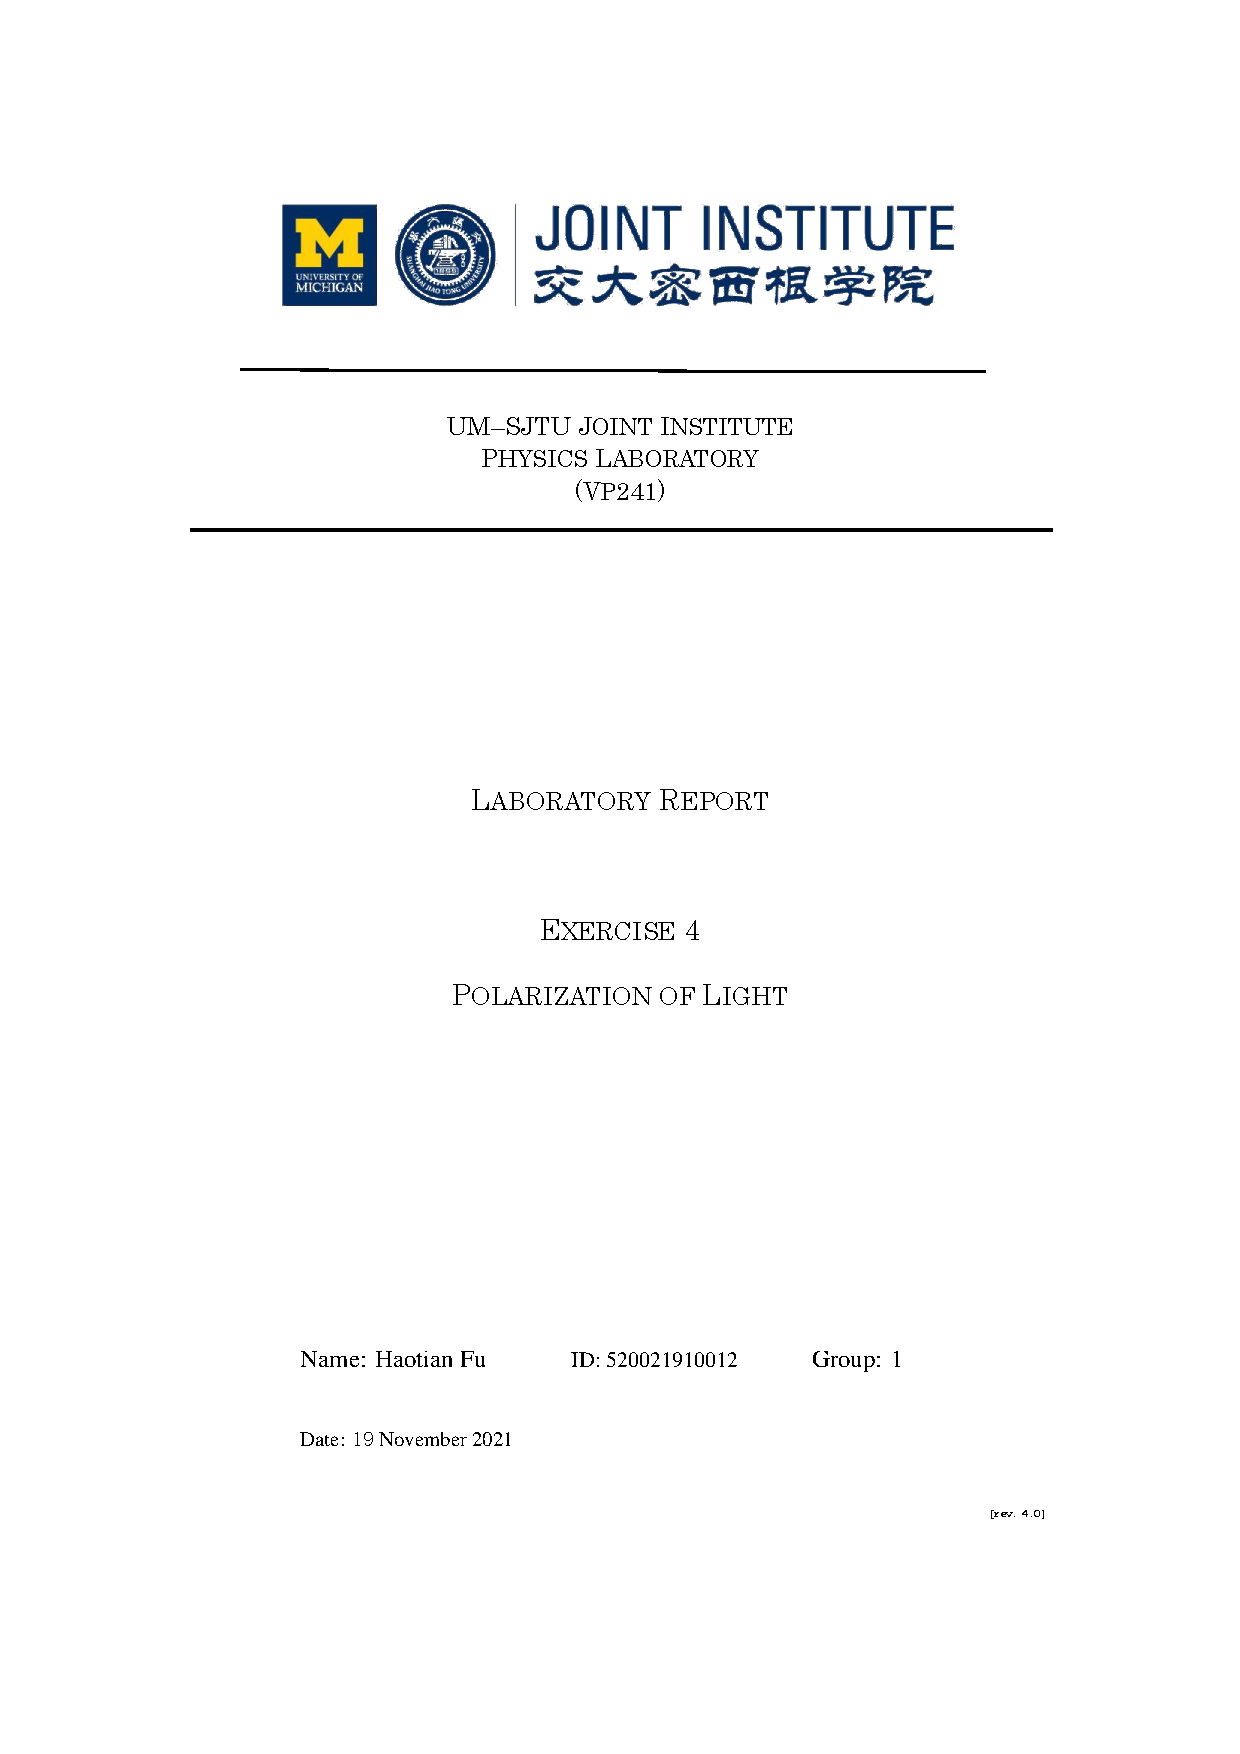
\includepdf{lab4_cover.pdf}

\newpage
\tableofcontents
\setcounter{page}{1}

\newpage
\listoffigures
\listoftables

\newpage
\section{Introduction}
The objective of this exercise is to understand some properties of light, in particular to study the polarization phenomenon.
Here we will also verify Malus’ law, as well as to understand the way half- and quarter-wave plates work in optical systems.
Besides, some investigation of elliptically and circularly polarized light will be generated and detected.

\subsection{Basic Concepts}
\begin{itemize}
	\item \textbf{Polarization:}$^{[1]}$ Polarization (also polarisation) is a property applying to transverse waves that specifies the geometrical orientation of the oscillations. In a transverse wave, the direction of the oscillation is perpendicular to the direction of motion of the wave..

	\item \textbf{Polarizer:}$^{[2]}$ A polarizer or polariser is an optical filter that lets light waves of a specific polarization pass through while blocking light waves of other polarizations.
	      \begin{figure}[!htbp]
		      \centering
		      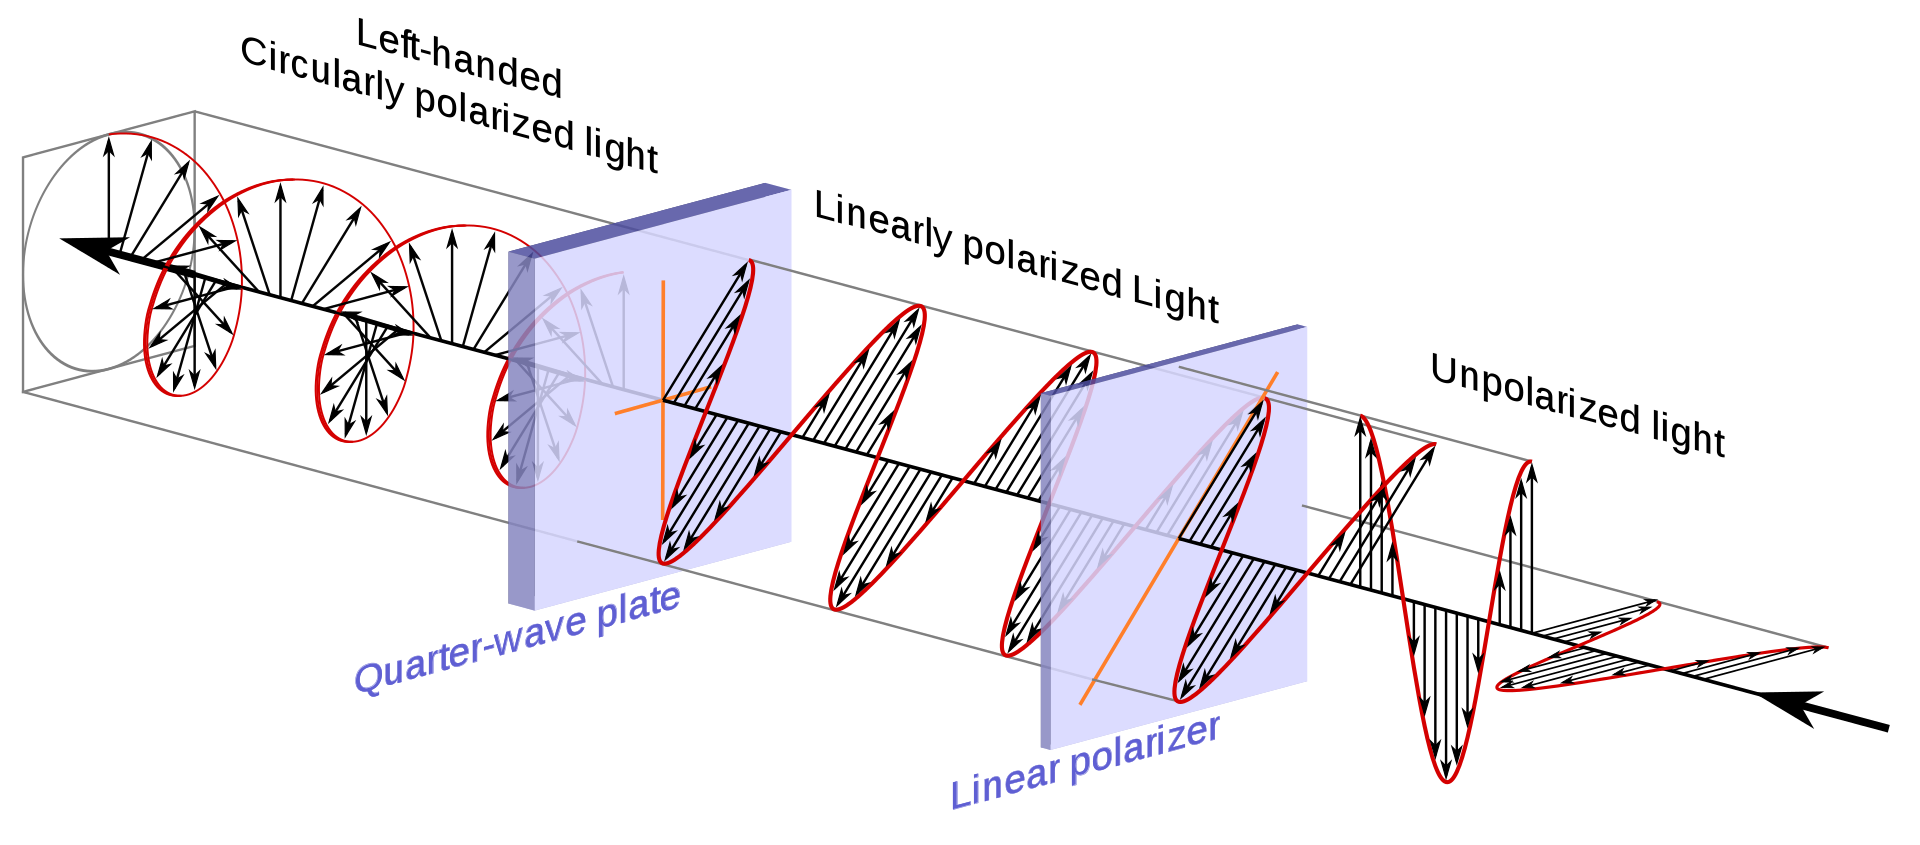
\includegraphics[width=0.6\textwidth]{polarizer.png}
		      \caption{Polarizer}
	      \end{figure}

	\item \textbf{Malus’ law:}$^{[3]}$ Malus’ law states that the intensity of plane-polarized light that passes through an analyzer varies as the square of the cosine of the angle between the plane of the polarizer and the transmission axes of the analyzer.
	      \begin{equation}
		      I_{\text {light }}=I_{\text {light }, 0} \cos ^{2} \theta
		      \label{eq::Malus’ law}
	      \end{equation}
	      where $I_{\text {light }, 0}$ is the intensity of the linearly polarized light incident on the analyzer.
	      \begin{figure}[!htbp]
		      \centering
		      \includegraphics[width=0.5\textwidth]{Malus’ law.png}
		      \caption{Change in the brightness of the light depends on the mutual orientation of the polarizer and the analyzer.}
		      \label{fig::Malus’ law}
	      \end{figure}
\end{itemize}

\subsection{Theoretical Basis}

\subsubsection{Polarization of Light$^{[3]}$}

\par Light in nature is electromagnetic wave. The electric field vector \textbf{E} in the electromagnetic wave is referred to as the light vector.
Light emitted from ordinary light sources (natural light) is unpolarized. However it can be regarded as a statistical equal-weight mixture of linearly
polarized waves with equal amplitudes. There the light may be also partially polarized, which means it can be regarded as a combination of a polarized
and the natural (unpolarized) light. The direction corresponding to the maximum amplitude of the light vector of such partially polarized light is the
oscillation direction of the polarized component.

\begin{figure}[!htbp]
	\centering
	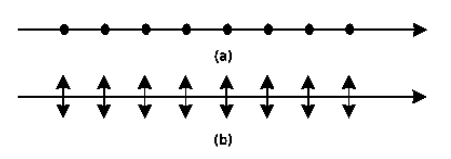
\includegraphics[width=0.6\textwidth]{polarization of light.png}
	\caption{(a) Linearly polarized light with the polarization axis perpendicular to the page
		plane. (b) Linearly polarized light with the polarization axis parallel to the page plane.}
	\label{fig::polarization of light}
\end{figure}


\subsubsection{Generation of Elliptically and Circularly Polarized Light. Half-wave and Quarter-wave Plates}
\par Suppose that linearly polarized light is incident normally on a crystal plate whose surface is parallel to its optical axis, and the angle between the polarizing
axis and the optical axis of the plate is $\alpha$. Then the linearly polarized light is resolved into two waves: an $e$-wave with the oscillation direction parallel
to the optical axis of the plate (extraordinary axis) and an o-wave whose oscillation direction is perpendicular to the optical axis (ordinary axis). They propagate in
the same direction, but with different speeds. The resulting optical path difference over the thickness $d$ of the plate is
\begin{equation}
	\Delta=\left(n_{\mathrm{e}}-n_{\mathrm{o}}\right) d
\end{equation}
and, consequently, the phase difference
\begin{equation}
	\delta=\frac{2 \pi}{\lambda}\left(n_{\mathrm{e}}-n_{\mathrm{o}}\right) d
\end{equation}
where $\lambda$ is the wavelength, $n_{\mathrm{e}}$ is the refractive index for the extraordinary axis, and $n_{\mathrm{o}}$ is the refractive index for the ordinary axis.
In a so-called positive crystal $\delta>0$, whereas in a negative one $\delta<0$.

\begin{figure}[!htbp]
	\centering
	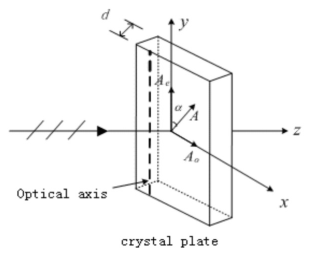
\includegraphics[width=0.5\textwidth]{waveplate.png}
	\caption{Linearly polarized light passing through a waveplate.}
	\label{fig::waveplate}
\end{figure}

As shown in Fig.(\ref{fig::waveplate}) , when the light propagates through the crystal plate, the two components of the light vector are

\begin{align*}
	E_{x} & =A_{\mathrm{o}} \cos \omega t          \\
	E_{y} & =A_{\mathrm{e}} \cos (\omega t+\delta)
\end{align*}

where $A_{\mathrm{e}}=A \cos \alpha, A_{\mathrm{o}}=A \sin \alpha$. Eliminating time from the above equations one obtains

\begin{equation}
	\frac{E_{x}^{2}}{A_{\mathrm{o}}^{2}}+\frac{E_{y}^{2}}{A_{\mathrm{e}}^{2}}-2 \frac{E_{x} E_{y}}{A_{\mathrm{o}} A_{\mathrm{e}}} \cos \delta=\sin ^{2} \delta
	\label{eq::equation of an ellipse}
\end{equation}

Note that is the equation of an ellipse for $\delta=\pm \pi / 2$.
When the thickness of the plate changes, the optical path difference changes as well. Some cases of particular interest, are discussed below:

$\blacktriangleright$ If $\Delta=k \lambda$, where $k=0,1,2, \ldots$, the phase difference $\delta=0$, and Eq.(\ref{eq::equation of an ellipse}) reduces to
$$
	E_{y}=\frac{A_{\mathrm{e}}}{A_{\mathrm{o}}} E_{x}
$$
which is a linear equation. Hence the transmitted light is linearly polarized with the oscillation direction remaining unchanged. A waveplate that satisfies
this condition is called a full-wave plate. The light goes through a full-wave plate without changing its polarization state.

$\blacktriangleright$ If $\Delta=(2 k+1) \lambda / 2$, where $k=0,1,2, \ldots$, the phase difference $\delta=\pi$, and Eq.(\ref{eq::equation of an ellipse})
simplifies to
$$
	E_{y}=-\frac{A_{\mathrm{e}}}{A_{\mathrm{o}}} E_{x}
$$
The transmitted light is also linearly polarized with the polarization axis rotated by the angle of $2 \alpha$. A waveplate that satisfies the condition is called
$1 / 2$-wave plate or half-wave plate. When a polarized light passes through a half-wave plate, its polarization axis gets rotated by an angle $2 \alpha$. If
$\alpha=\pi / 4$, then the polarization axis of the transmitted light is perpendicular to that of the incident light.

$\blacktriangleright$ Finally, if $\Delta=(2 k+1) \lambda / 4$, where $k=0,1,2, \ldots$, the phase difference $\delta=\pm \pi / 2$ and Eq. (2) transforms into
$$
	\frac{E_{x}^{2}}{A_{\mathrm{o}}^{2}}+\frac{E_{y}^{2}}{A_{\mathrm{e}}^{2}}=1
$$
The transmitted light is elliptically polarized. A waveplate that satisfies the above condition is called a $1 / 4$-wave plate or a quarter-waveplate and is an
important optical element in many polarization experiments.

If $A_{\mathrm{e}}=A_{\mathrm{o}}=A$, then $E_{x}^{2}+E_{y}^{2}=A^{2}$, and the transmitted light is circularly polarized. Since the amplitudes of the
$o$-wave and the $e$-wave are both functions of $\alpha$, the polarization state after passing through a $1 / 4$-wave plate will vary, depending on the angle:
$\blacktriangleright$ if $\alpha=0$, the transmitted light is linearly polarized with the polarization axis parallel to the optical axis of the $1 / 4$-wave plate;
$\blacktriangleright$ if $\alpha=\pi / 2$, the transmitted light is linearly polarized with the polarization axis perpendicular to the optical axis of the $1 / 4$-wave plate;
$\blacktriangleright$ if $\alpha=\pi / 4$, the transmitted light is circularly polarized;
$\blacktriangleright$ otherwise, the transmitted light is elliptically polarized.

\section{Apparatus and Measurement Procedure}

\subsection{Apparatus}
The measurement setup consists of: a semiconductor laser, a tungsten iodine lamp,
a silicon photo-cell, a UT51 digital universal meter, as well as two polarizers, 1/2-wave
and 1/4-wave plates (the uncertainty of the the angle is 2$^\circ$) and a lens with a glass sheet.
The elements are placed on an optical bench.

The precisions of the devices are shown in Table \ref{table::Precision}.
\begin{table}[htbp]
	\centering
	\begin{tabular}{cc}
		\hline
		Instrument & Uncertainties    \\
		\hline
		Angle      & $\pm 2^\circ$    \\
		Current    & $\pm 0.01\ \mu$A \\
		\hline
	\end{tabular}
	\caption{Information of measurement instruments.}
	\label{table::Precision}
\end{table}

\begin{figure}[!htbp]
	\centering
	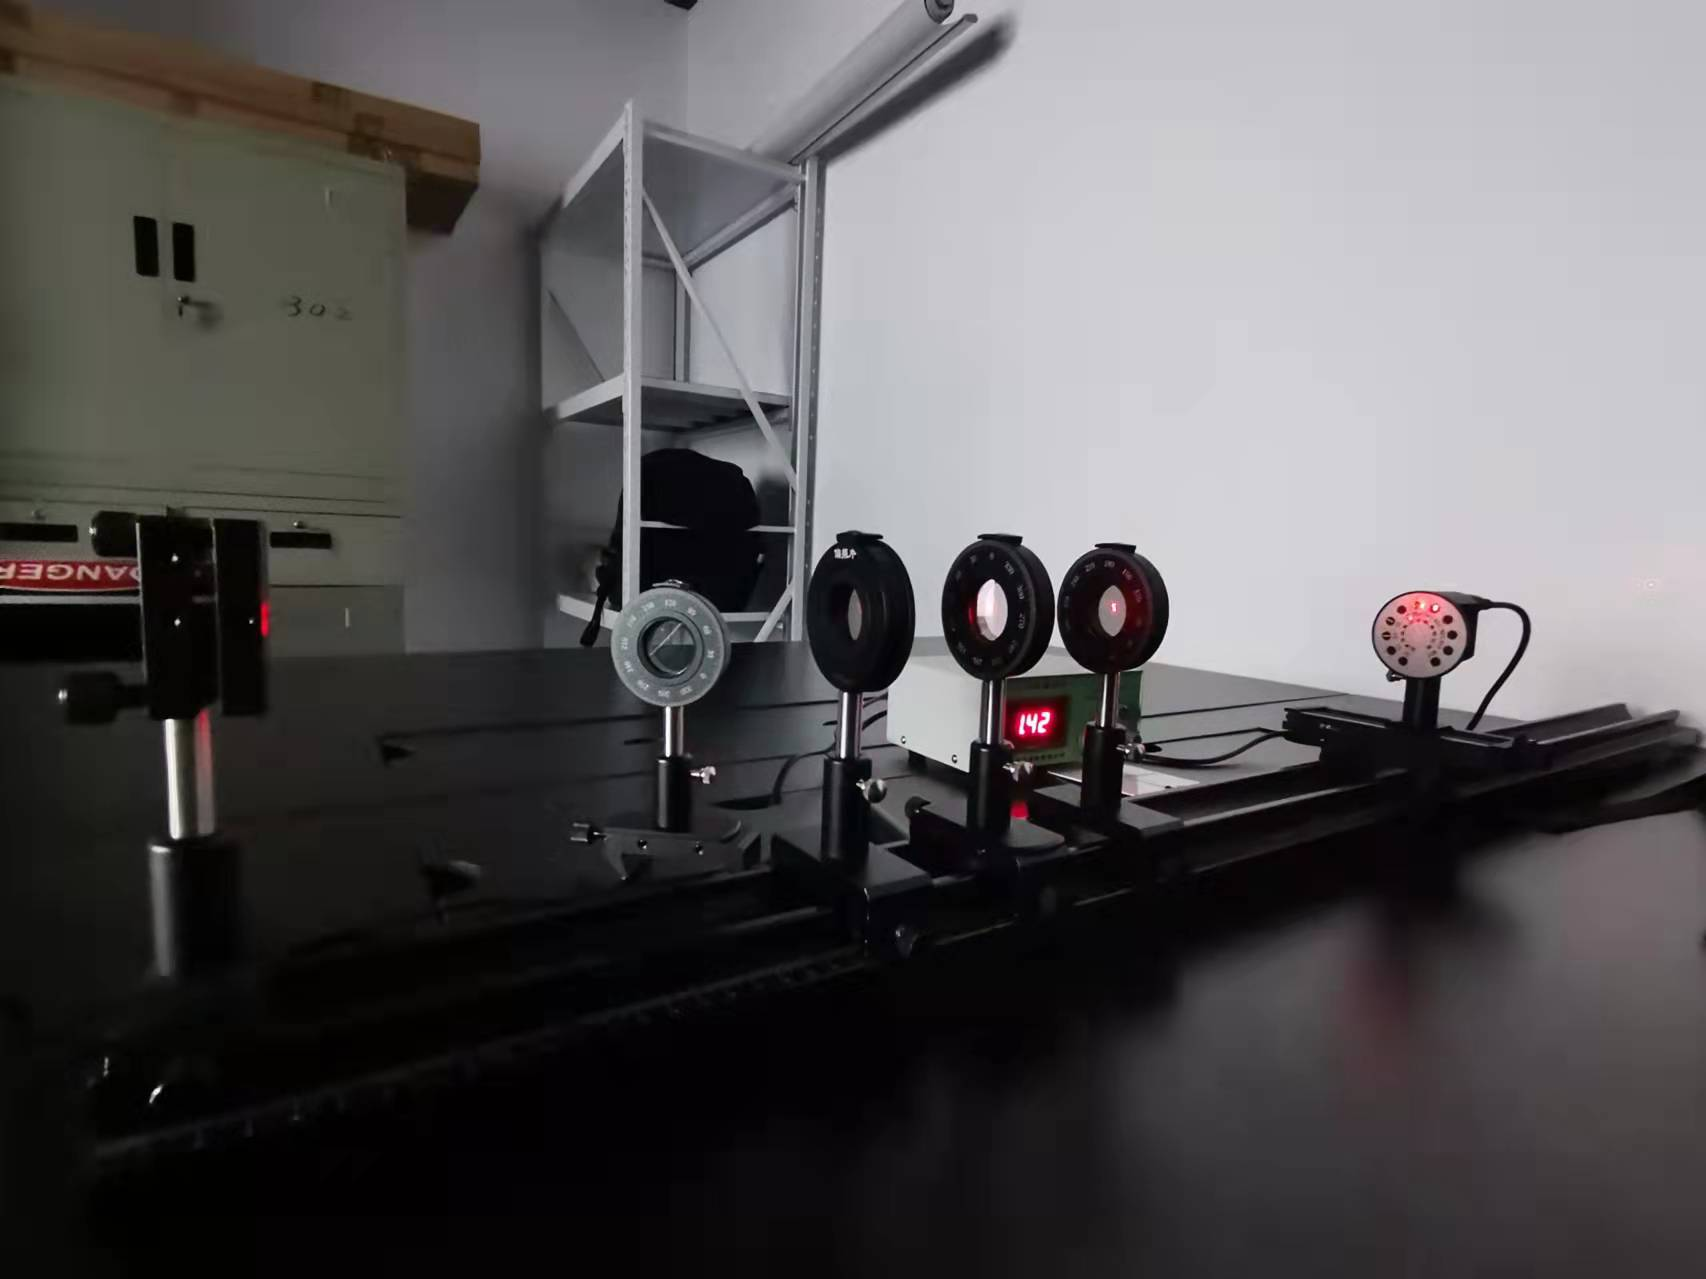
\includegraphics[width=0.5\textwidth]{apparatus.jpg}
	\caption{Apparatus}
\end{figure}

\subsection{Measurement Procedure}

\subsubsection{Apparatus Adjustment}
\begin{enumerate}[a.]
	\item Adjust the laser and the photo-cell so that the light can pass through the $\phi$ 6.0 aperture.
	\item Placed the analyzer onto the optical bench, adjust its position so that the current detected is in the range 0.8 $\sim$ 1.8 $\mu$A.
\end{enumerate}

\subsubsection{Demonstration of Malus' Law}
\begin{enumerate}[a.]
	\item Place an analyzer between the polarizer and the photo-cell. Record this value as $I_0$.
	\item Adjust the angle of the analyzer until the electric current reaches 0. Set this position as $\theta = 90^\circ$.
	\item Rotate the analyzer from $90^\circ$ to $0^\circ$ and record the magnitude of the current $I$ every $5^\circ$ and record the values.
	\item To verify Malus' Law, plot the graph $I/I_0$ vs. $\cos^2\theta$ and perform linear fitting.
\end{enumerate}

\subsubsection{Linearly Polarized Light and the Half-wave Plate}
\begin{enumerate}[a.]
	\item Place the 1/2-wave plate between the polarizer and the analyzer. Rotate it to make the light extinction appear again and set this position as the initial position.
	\item Rotate the 1/2-wave plate for $\alpha = 10^\circ$ from the initial position and rotate the analyzer to make the light extinction appear again, record the angle of rotation $\Delta\theta$.
	\item To explore the relationship, plot the graph $\Delta\theta$ vs. $\theta$.
\end{enumerate}

\subsubsection{Circularly and Elliptically Polarized Light and the 1/4-wave Plate}
\begin{enumerate}[a.]
	\item Replace the 1/2-wave plate by the 1/4-wave plate and rotate it to make the light extinction appear and set this position as the initial position. At this point $\alpha = 0^\circ$. Then rotate the 1/4-wave plate and observe the change in the light intensity.
	\item Rotate the analyzer for $360^\circ$ and record the light intensity (which is indicated by the current $I$) for every $10^\circ$ and record the data in a table.
	\item Rotate the 1/4-wave plate for $20^\circ$, repeat Step 3.
	\item Rotate the 1/4-wave plate for $45^\circ$, and repeat Step 3.
	\item Rotate the 1/4-wave plate for $70^\circ$. Rotate the analyzer and record its position and the magnitude of the current when the light intensity reaches a maximum.
	\item To find out the relation, plot the relation between the rotation angle of the analyzer and the light amplitude in polar coordinates. Normalize the amplitude by its maximum value. Mark the position recorded in Step 6 and compare it with the data recorded.
	\item To compare with the circular polarization, plot a linear fit to the data when the angle is $45^\circ$.
\end{enumerate}

\subsection{Safety Notice}

\begin{enumerate}[a.]
	\item Do not direct the laser beam into the eye.
	\item Do not touch the surface of the polarizers or the wave plates.
	\item Please leave the equipment in order before leaving.
\end{enumerate}


\section{Experimental Results}

\subsection{Demonstration of Malus' Law}
The measurement data are presented in Table \ref{table::Malus_Measure}.

\begin{table}[H]\centering
	\begin{tabular}{cc||cc}
		\hline
		\multicolumn{2}{c}{Maximum Electric Current $I_0$} & \multicolumn{2}{c}{2.21 $\pm$ 0.01 [$\mu$A]}                                                                                         \\
		\hline
		$\theta\,\,[^\circ] \pm 2[^\circ]$                 & $I\,\,[\mu\text{A}] \pm 0.01\,\,[\mu\text{A}]$ & $\theta\,\,[^\circ] \pm 2[^\circ]$ & $I\,\,[\mu\text{A}] \pm 0.01\,\,[\mu\text{A}]$ \\
		\hline
		0                                                  & 2.21                                           & 50                                 & 0.96                                           \\
		5                                                  & 2.20                                           & 55                                 & 0.77                                           \\
		10                                                 & 2.16                                           & 60                                 & 0.58                                           \\
		15                                                 & 2.09                                           & 65                                 & 0.42                                           \\
		20                                                 & 1.99                                           & 70                                 & 0.30                                           \\
		25                                                 & 1.89                                           & 75                                 & 0.17                                           \\
		30                                                 & 1.75                                           & 80                                 & 0.08                                           \\
		35                                                 & 1.57                                           & 85                                 & 0.03                                           \\
		40                                                 & 1.37                                           & 90                                 & 0.00                                           \\
		45                                                 & 1.17                                           &                                    &                                                \\
		\hline
	\end{tabular}
	\caption{Measurement data for Malus' law demonstration.}
	\label{table::Malus_Measure}
\end{table}

To find the relation between $\cos^2\theta$ and $I/I_0$, the two set of values need to be calculated first.
Take the first set of data as an example.
$$\cos^2\theta = \cos^2(0 \times \frac{\pi}{180}) = 1 \pm 0,$$
$$\frac{I}{I_0} = \frac{2.21}{2.21} = 1.000 \pm 0.006.$$
Perform similar calculations to each of the other sets of data and the results are shown in Table \ref{table::cosine}.

\begin{table}[H]
	\centering
	\begin{tabular}{cccc}
		\hline
		$\theta\,\,[^\circ] \pm 2\,\,[^\circ]$ & $I\,\,[\mu\text{A}] \pm 0.01\,\,[\mu\text{A}]$ & $\cos^2\theta$     & $I/I_0$            \\
		\hline
		0                                      & 2.21                                           & 1 $\pm$ 0          & 1.000  $\pm$ 0.006 \\
		5                                      & 2.20                                           & 0.992  $\pm$ 0.006 & 0.995  $\pm$ 0.006 \\
		10                                     & 2.16                                           & 0.970  $\pm$ 0.012 & 0.977  $\pm$ 0.006 \\
		15                                     & 2.09                                           & 0.93  $\pm$ 0.02   & 0.946  $\pm$ 0.006 \\
		20                                     & 1.99                                           & 0.88  $\pm$ 0.02   & 0.900  $\pm$ 0.006 \\
		25                                     & 1.89                                           & 0.82  $\pm$ 0.03   & 0.855  $\pm$ 0.006 \\
		30                                     & 1.75                                           & 0.75  $\pm$ 0.03   & 0.792  $\pm$ 0.006 \\
		35                                     & 1.57                                           & 0.67  $\pm$ 0.03   & 0.710  $\pm$ 0.006 \\
		40                                     & 1.37                                           & 0.59  $\pm$ 0.03   & 0.620  $\pm$ 0.005 \\
		45                                     & 1.17                                           & 0.50  $\pm$ 0.03   & 0.529  $\pm$ 0.005 \\
		50                                     & 0.96                                           & 0.41  $\pm$ 0.03   & 0.434  $\pm$ 0.005 \\
		55                                     & 0.77                                           & 0.33  $\pm$ 0.03   & 0.348  $\pm$ 0.005 \\
		60                                     & 0.58                                           & 0.25  $\pm$ 0.03   & 0.262  $\pm$ 0.005 \\
		65                                     & 0.42                                           & 0.18  $\pm$ 0.03   & 0.190  $\pm$ 0.005 \\
		70                                     & 0.30                                           & 0.12  $\pm$ 0.02   & 0.136  $\pm$ 0.005 \\
		75                                     & 0.17                                           & 0.07  $\pm$ 0.02   & 0.077  $\pm$ 0.005 \\
		80                                     & 0.08                                           & 0.030  $\pm$ 0.012 & 0.036  $\pm$ 0.005 \\
		85                                     & 0.03                                           & 0.008  $\pm$ 0.006 & 0.014  $\pm$ 0.005 \\
		90                                     & 0.00                                           & 0      $\pm$ 0     & 0.000  $\pm$ 0.005 \\
		\hline
	\end{tabular}
	\caption{Result for $\cos^2\theta$ and $I/I_0$.}
	\label{table::cosine}
\end{table}

Then, a linear fit of the plot $I/I_0$ vs. $\theta$ are performed (Fig.\ref{fig::Malus Law}). The slope of the linear fitting is 1.009 $\pm$ 0.004.

\begin{figure}[H]
	\centering
	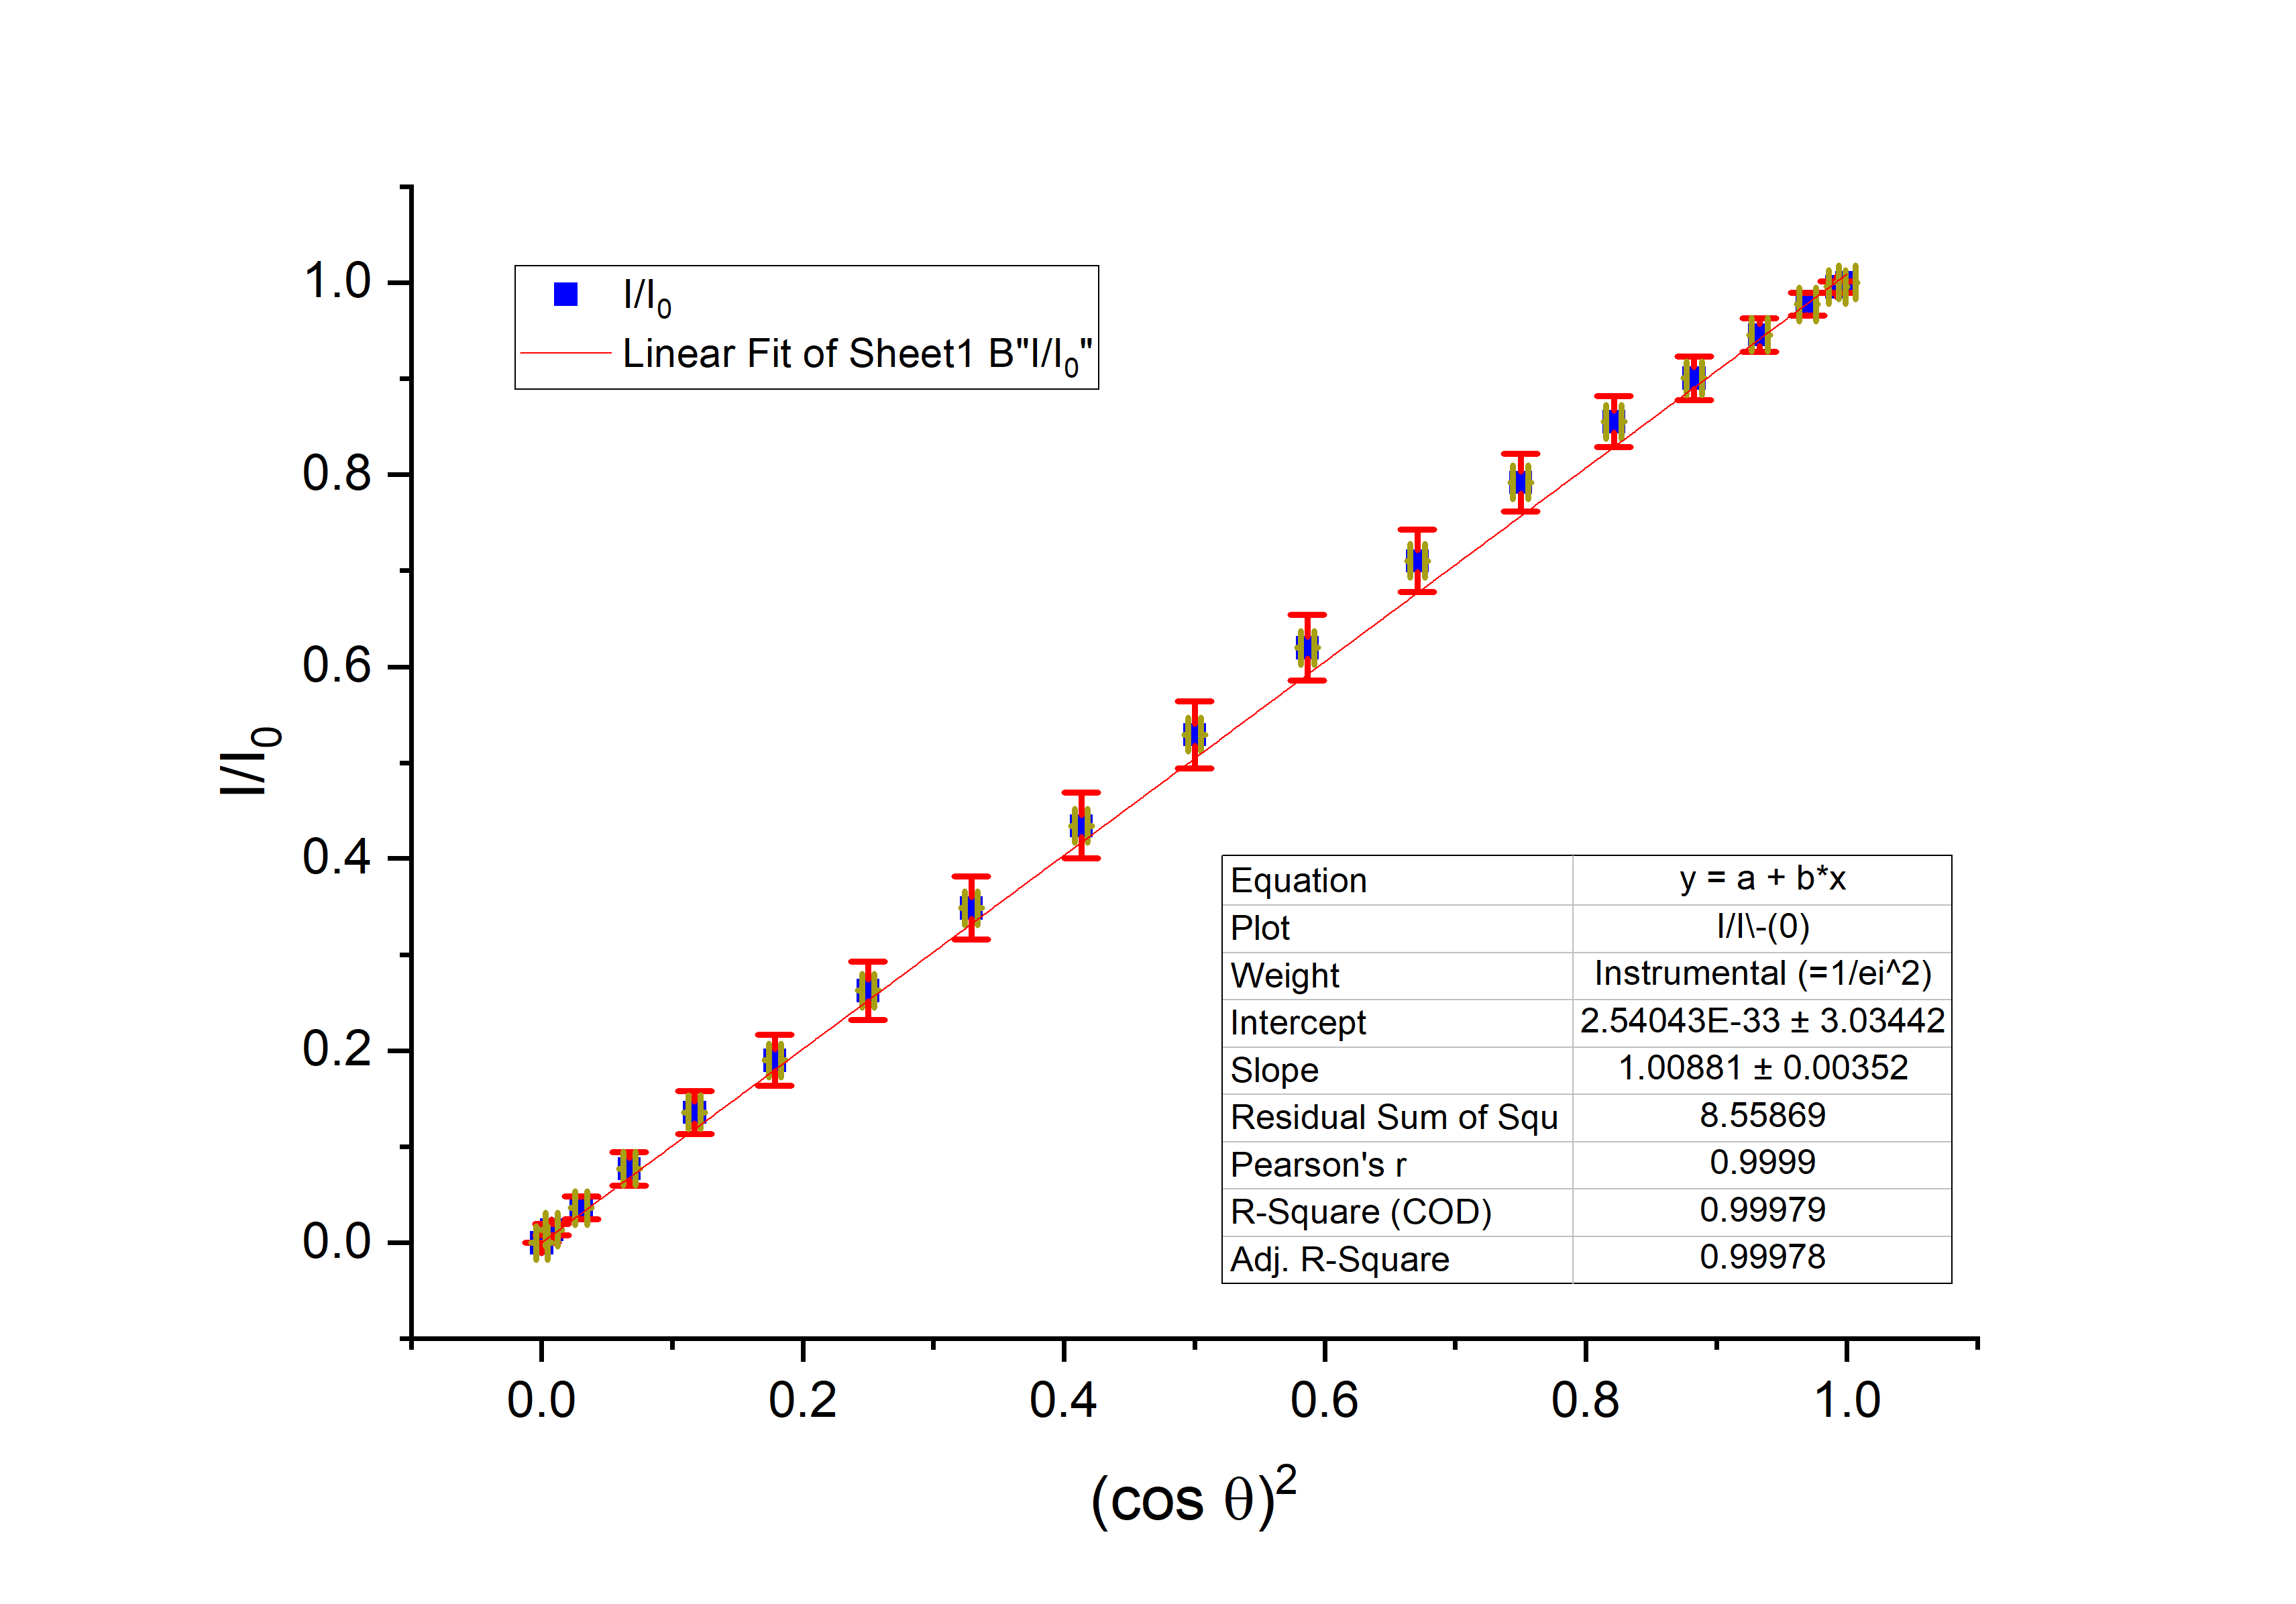
\includegraphics[scale=0.5]{Linear fit_Malus law.png}
	\caption{Linear fit of $I/I_0$ vs. $\cos^2\theta$ relation.}
	\label{fig::Malus Law}
\end{figure}

\subsection{Linearly Polarized Light and the Half-wave Plate}

The measurement data are presented in Table \ref{table::1/2}. Note that we have substracted each of the data by the initial angle in the report.

\begin{table}[H]
	\centering
	\begin{tabular}{cc}
		\hline
		Rotation angle of the 1/2-wave plate $[^\circ] \pm 2[^\circ]$ & Rotation angle of the analyzer $[^\circ] \pm 2[^\circ]$ \\
		\hline
		initial                                                       & 0                                                       \\
		10                                                            & 20                                                      \\
		20                                                            & 42                                                      \\
		30                                                            & 59                                                      \\
		40                                                            & 83                                                      \\
		50                                                            & 100                                                     \\
		60                                                            & 121                                                     \\
		70                                                            & 142                                                     \\
		80                                                            & 159                                                     \\
		90                                                            & 179                                                     \\
		\hline
	\end{tabular}
	\caption{Measurement data for the 1/2-wave plate.}
	\label{table::1/2}
\end{table}

To find the relation between $\Delta\theta$ and $\theta$, the data are plotted in Figure \ref{fig::delta} and linear fit is performed. The slope of the linear fit is $1.992 \pm 0.016$.

\begin{figure}[H]
	\centering
	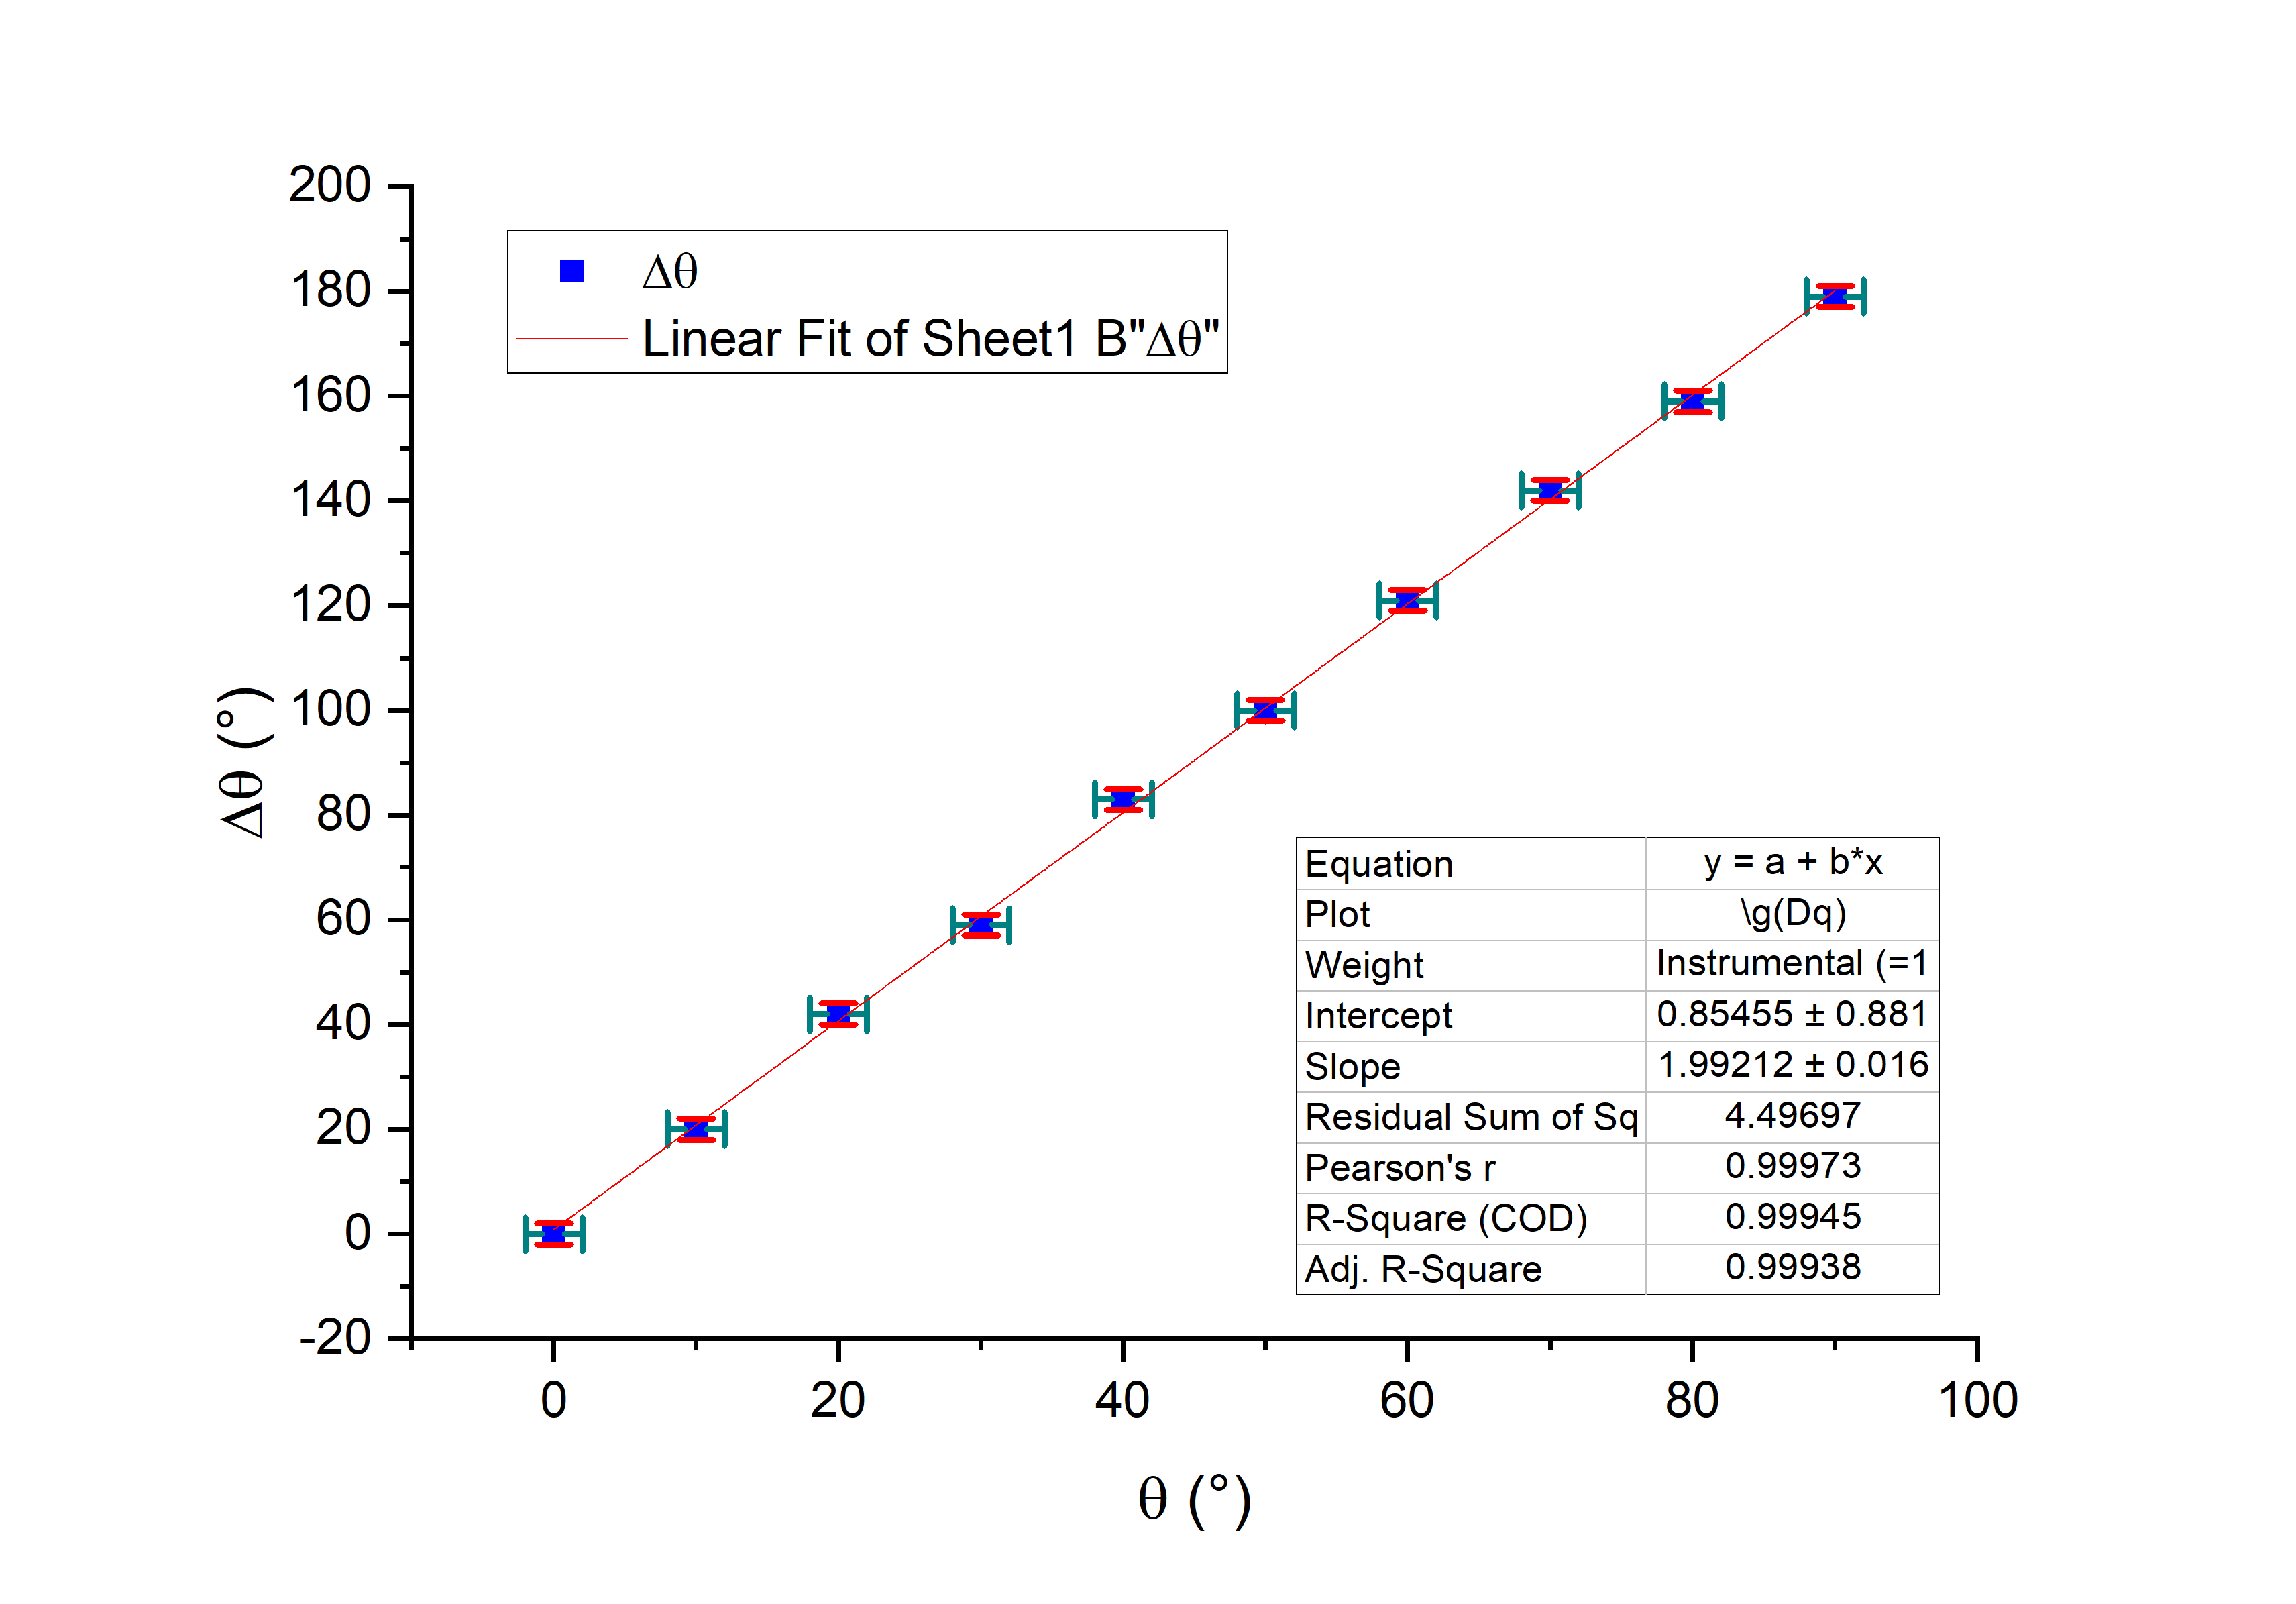
\includegraphics[scale=0.5]{delta.png}
	\caption{Linear fit of $\Delta\theta$ vs. $\theta$.}
	\label{fig::delta}
\end{figure}


Besides, in this part, when the half-wave plate rotates for 360$^\circ$, \textbf{4} times of light extinction are observed. And when the analyzer rotates 360$^\circ$,
\textbf{2} times of light extinction during the analyzer rotating 360$^\circ$. It can be concluded from the above result that
\textbf{the polarization axis get rotated by twice of the origin angle ($2\alpha$)} after the light passes through the 1/2-wave plate.

\subsection{Circularly and Elliptically Polarized Light and the 1/4-wave Plate}

\subsubsection{Rotation Angle: 0$^\circ$} \label{sec:0degree}

The measurement data for 0$^\circ$ rotation angle of 1/4-wave plate are presented in Table \ref{table::1/4,0}. Note that when filling the data sheet, 0$^\circ$ and 90 $^\circ$ are mistaken and the mistake is corrected in the report.

\begin{table}[H]
	\centering
	\begin{tabular}{cc||cc}
		\multicolumn{4}{c}{Rotation angle of 1/4-wave plate: 0$^\circ$}                                                                                                                           \\
		\hline
		\multicolumn{2}{c}{Maximum Electric Current $I_0$} & \multicolumn{2}{c}{1.48 $\pm$ 0.01 [$\mu$A]}                                                                                         \\
		\hline
		$\theta\,\,[^\circ] \pm 2[^\circ]$                 & $I\,\,[\mu\text{A}] \pm 0.01\,\,[\mu\text{A}]$ & $\theta\,\,[^\circ] \pm 2[^\circ]$ & $I\,\,[\mu\text{A}] \pm 0.01\,\,[\mu\text{A}]$ \\
		\hline
		0                                                  & 0.02                                           & 180                                & 0.02                                           \\
		10                                                 & 0.05                                           & 190                                & 0.06                                           \\
		20                                                 & 0.18                                           & 200                                & 0.17                                           \\
		30                                                 & 0.37                                           & 210                                & 0.38                                           \\
		40                                                 & 0.62                                           & 220                                & 0.62                                           \\
		50                                                 & 0.88                                           & 230                                & 0.88                                           \\
		60                                                 & 1.13                                           & 240                                & 1.11                                           \\
		70                                                 & 1.30                                           & 250                                & 1.29                                           \\
		80                                                 & 1.43                                           & 260                                & 1.41                                           \\
		90                                                 & 1.48                                           & 270                                & 1.48                                           \\
		100                                                & 1.39                                           & 280                                & 1.44                                           \\
		110                                                & 1.25                                           & 290                                & 1.35                                           \\
		120                                                & 1.10                                           & 300                                & 1.15                                           \\
		130                                                & 0.88                                           & 310                                & 0.90                                           \\
		140                                                & 0.62                                           & 320                                & 0.65                                           \\
		150                                                & 0.39                                           & 330                                & 0.41                                           \\
		160                                                & 0.20                                           & 340                                & 0.21                                           \\
		170                                                & 0.07                                           & 350                                & 0.08                                           \\
		\hline
	\end{tabular}
	\caption{Measurement data for the 1/4-wave plate (rotation angle 0$^\circ$).}
	\label{table::1/4,0}
\end{table}

As described in the procedure part, $\sqrt{I/I_0}$ is calculated. Take the first set of data as an example,
$$\sqrt{\frac{I}{I_0}} = \sqrt{\frac{0.02}{1.48}} = 0.12 \pm 0.03.$$
Perform similar calculations to each of the other sets of data and the results are presented in Table \ref{TableSqrt}.

\begin{table}[H]
	\centering
	\begin{tabular}{cc||cc}
		\hline
		$\theta\,\,[^\circ] \pm 2[^\circ]$ & $\sqrt{I/I_0}$       & $\theta\,\,[^\circ] \pm 2[^\circ]$ & $\sqrt{I/I_0}$      \\
		\hline
		0                                  & 0.12     $\pm$ 0.03  & 180                                & 0.12    $\pm$ 0.03  \\
		10                                 & 0.18     $\pm$ 0.02  & 190                                & 0.20    $\pm$ 0.02  \\
		20                                 & 0.349    $\pm$ 0.010 & 200                                & 0.339   $\pm$ 0.010 \\
		30                                 & 0.500    $\pm$ 0.007 & 210                                & 0.507   $\pm$ 0.007 \\
		40                                 & 0.647    $\pm$ 0.006 & 220                                & 0.647   $\pm$ 0.006 \\
		50                                 & 0.771    $\pm$ 0.005 & 230                                & 0.771   $\pm$ 0.005 \\
		60                                 & 0.874    $\pm$ 0.005 & 240                                & 0.866   $\pm$ 0.005 \\
		70                                 & 0.937    $\pm$ 0.005 & 250                                & 0.934   $\pm$ 0.005 \\
		80                                 & 0.983    $\pm$ 0.004 & 260                                & 0.976   $\pm$ 0.004 \\
		90                                 & 1.000    $\pm$ 0.004 & 270                                & 1.000   $\pm$ 0.004 \\
		100                                & 0.969    $\pm$ 0.004 & 280                                & 0.986   $\pm$ 0.004 \\
		110                                & 0.919    $\pm$ 0.005 & 290                                & 0.955   $\pm$ 0.004 \\
		120                                & 0.862    $\pm$ 0.005 & 300                                & 0.881   $\pm$ 0.005 \\
		130                                & 0.771    $\pm$ 0.005 & 310                                & 0.780   $\pm$ 0.005 \\
		140                                & 0.647    $\pm$ 0.006 & 320                                & 0.663   $\pm$ 0.006 \\
		150                                & 0.513    $\pm$ 0.007 & 330                                & 0.526   $\pm$ 0.007 \\
		160                                & 0.368    $\pm$ 0.010 & 340                                & 0.377   $\pm$ 0.009 \\
		170                                & 0.22     $\pm$ 0.02  & 350                                & 0.232   $\pm$ 0.015 \\
		\hline
	\end{tabular}
	\caption{Results for $\sqrt{I/I_0}$ when rotation angle is 0$^\circ$.}
	\label{TableSqrt}
\end{table}

Then the relationship of $\sqrt{I/I_0}$ and $\theta$ are plotted in polar coordinate (Fig.\ref{fig::0degree}).

\begin{figure}[H]
	\centering
	\subfigure[$\sqrt{I/I_0}$ vs. $\theta$ relation in polar coordinate when rotation angle is 0$^\circ$.]{
    	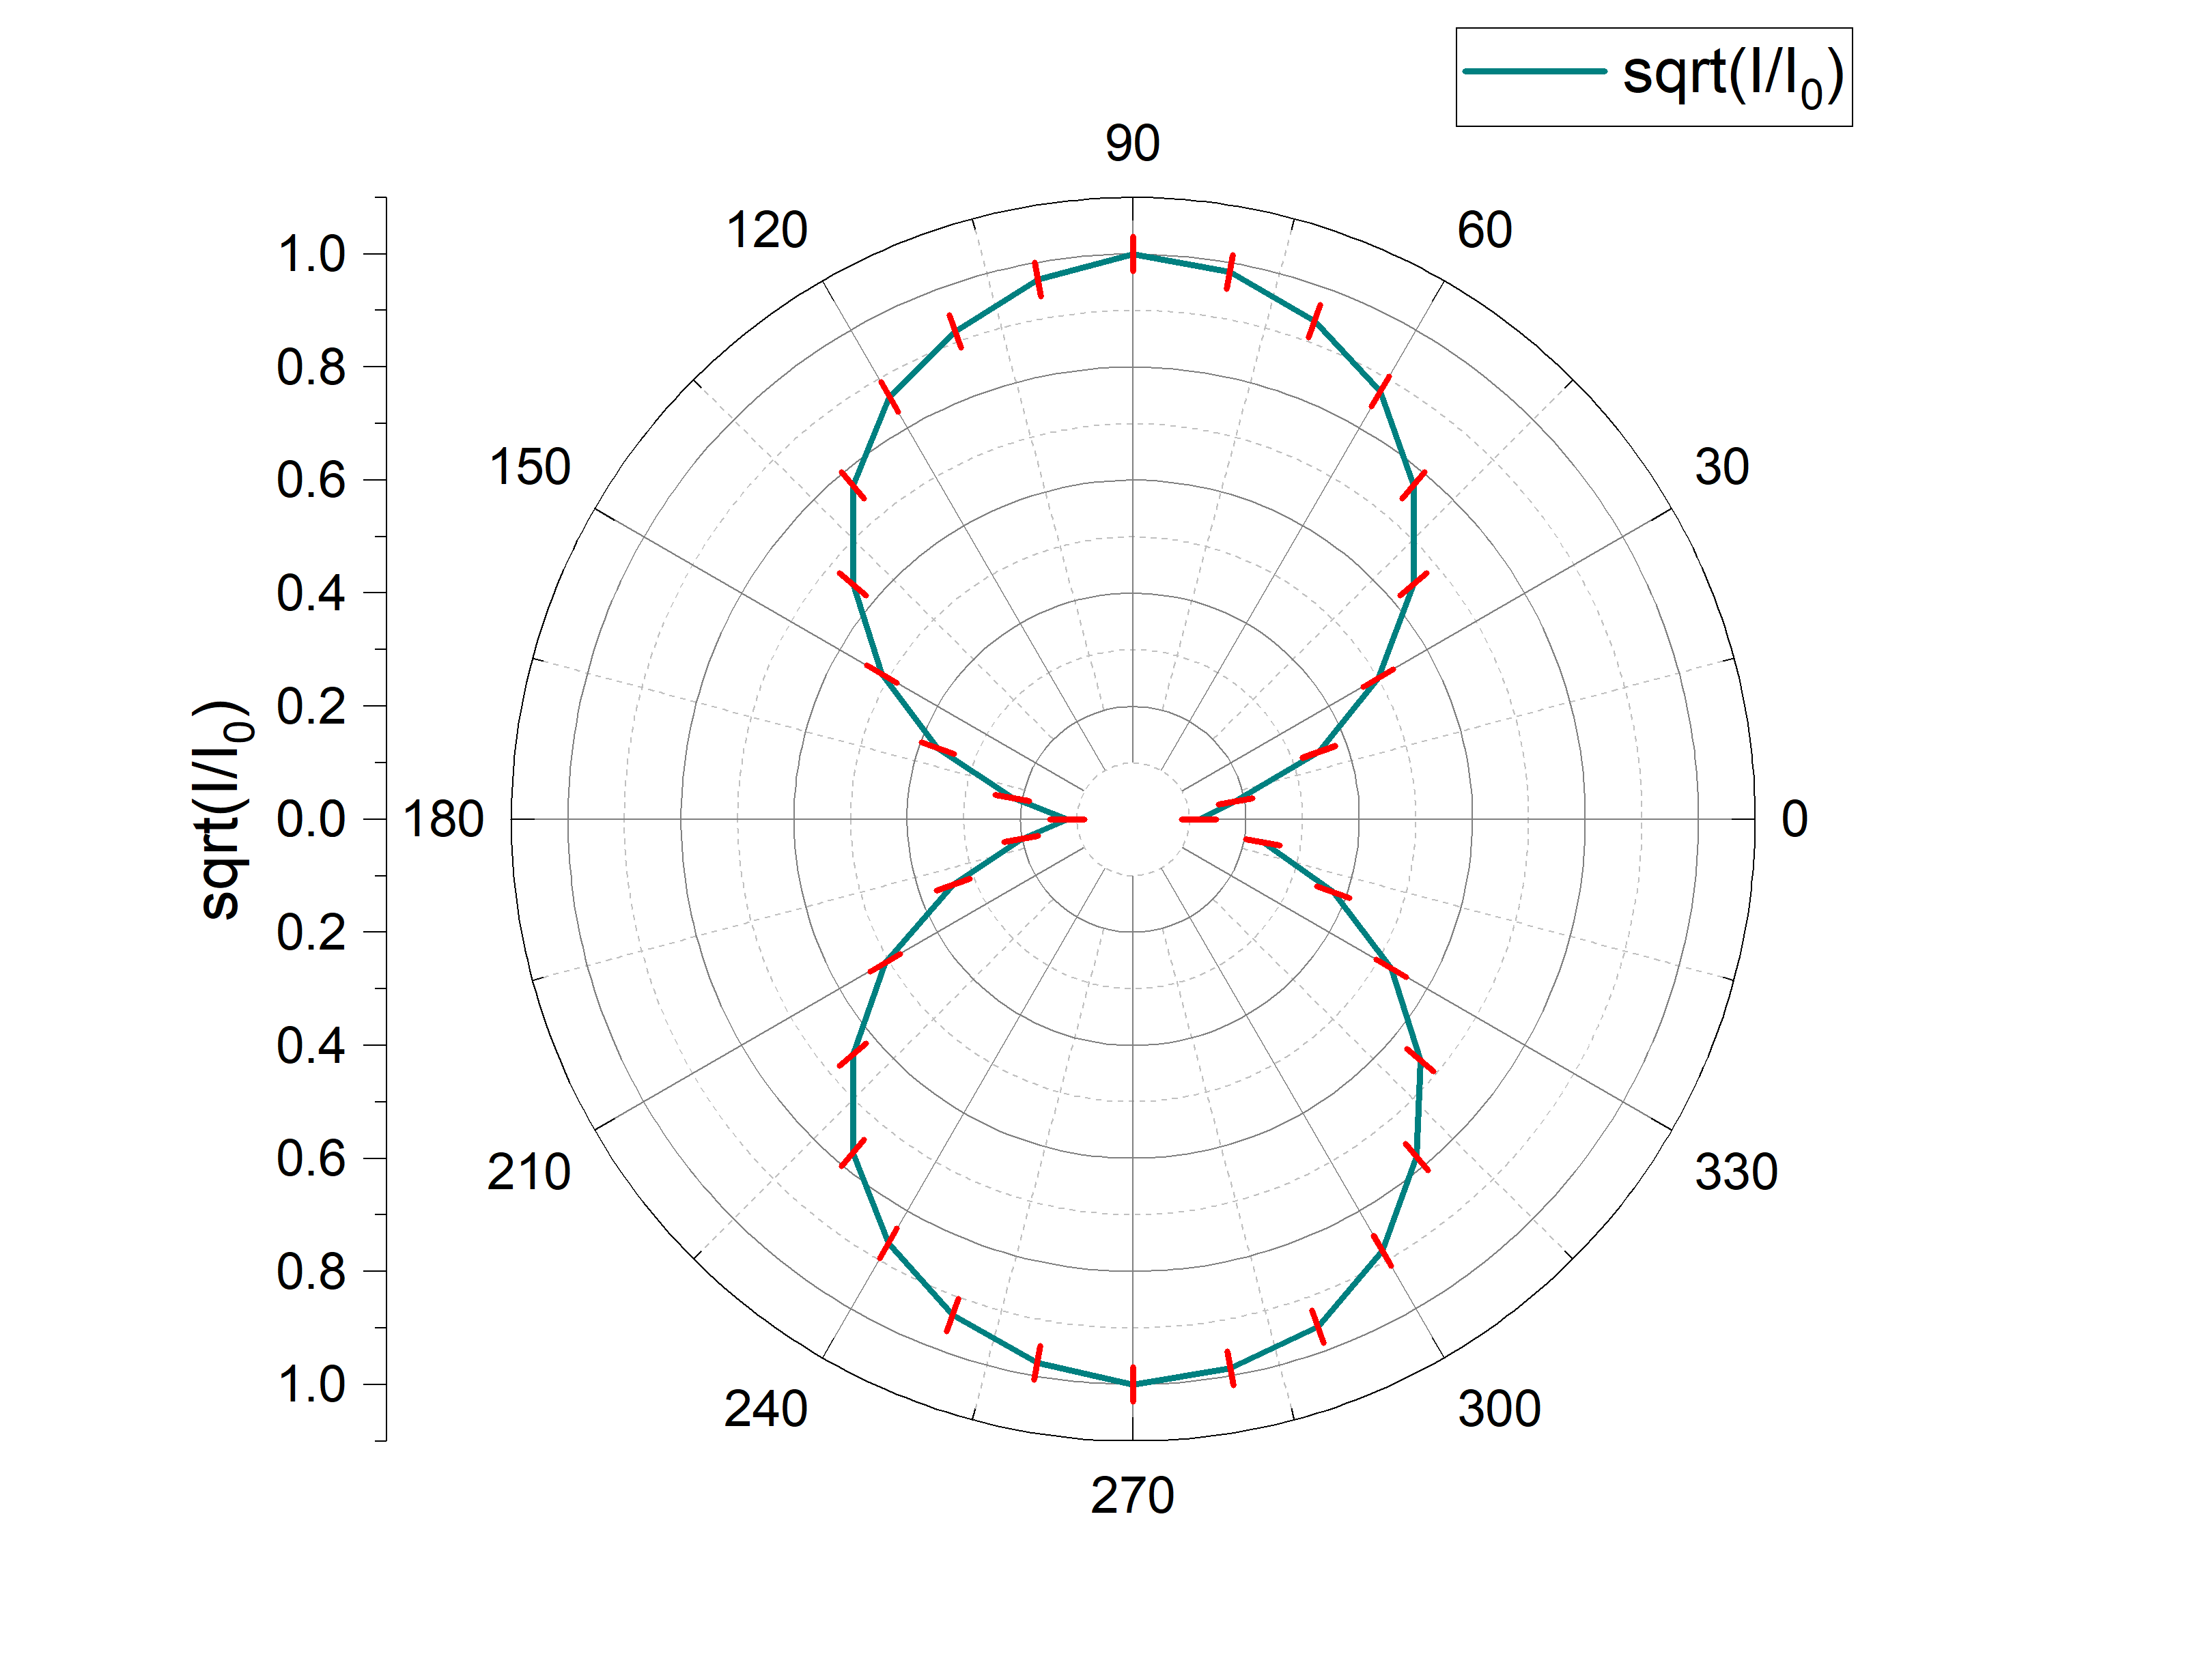
\includegraphics[width=0.45\textwidth]{00.png}
    }\hspace{5mm}
	\subfigure[$\sqrt{I/I_0}$ vs. $\theta$ relation in Cartesian coordinate when rotation angle is 0$^\circ$.]{
    	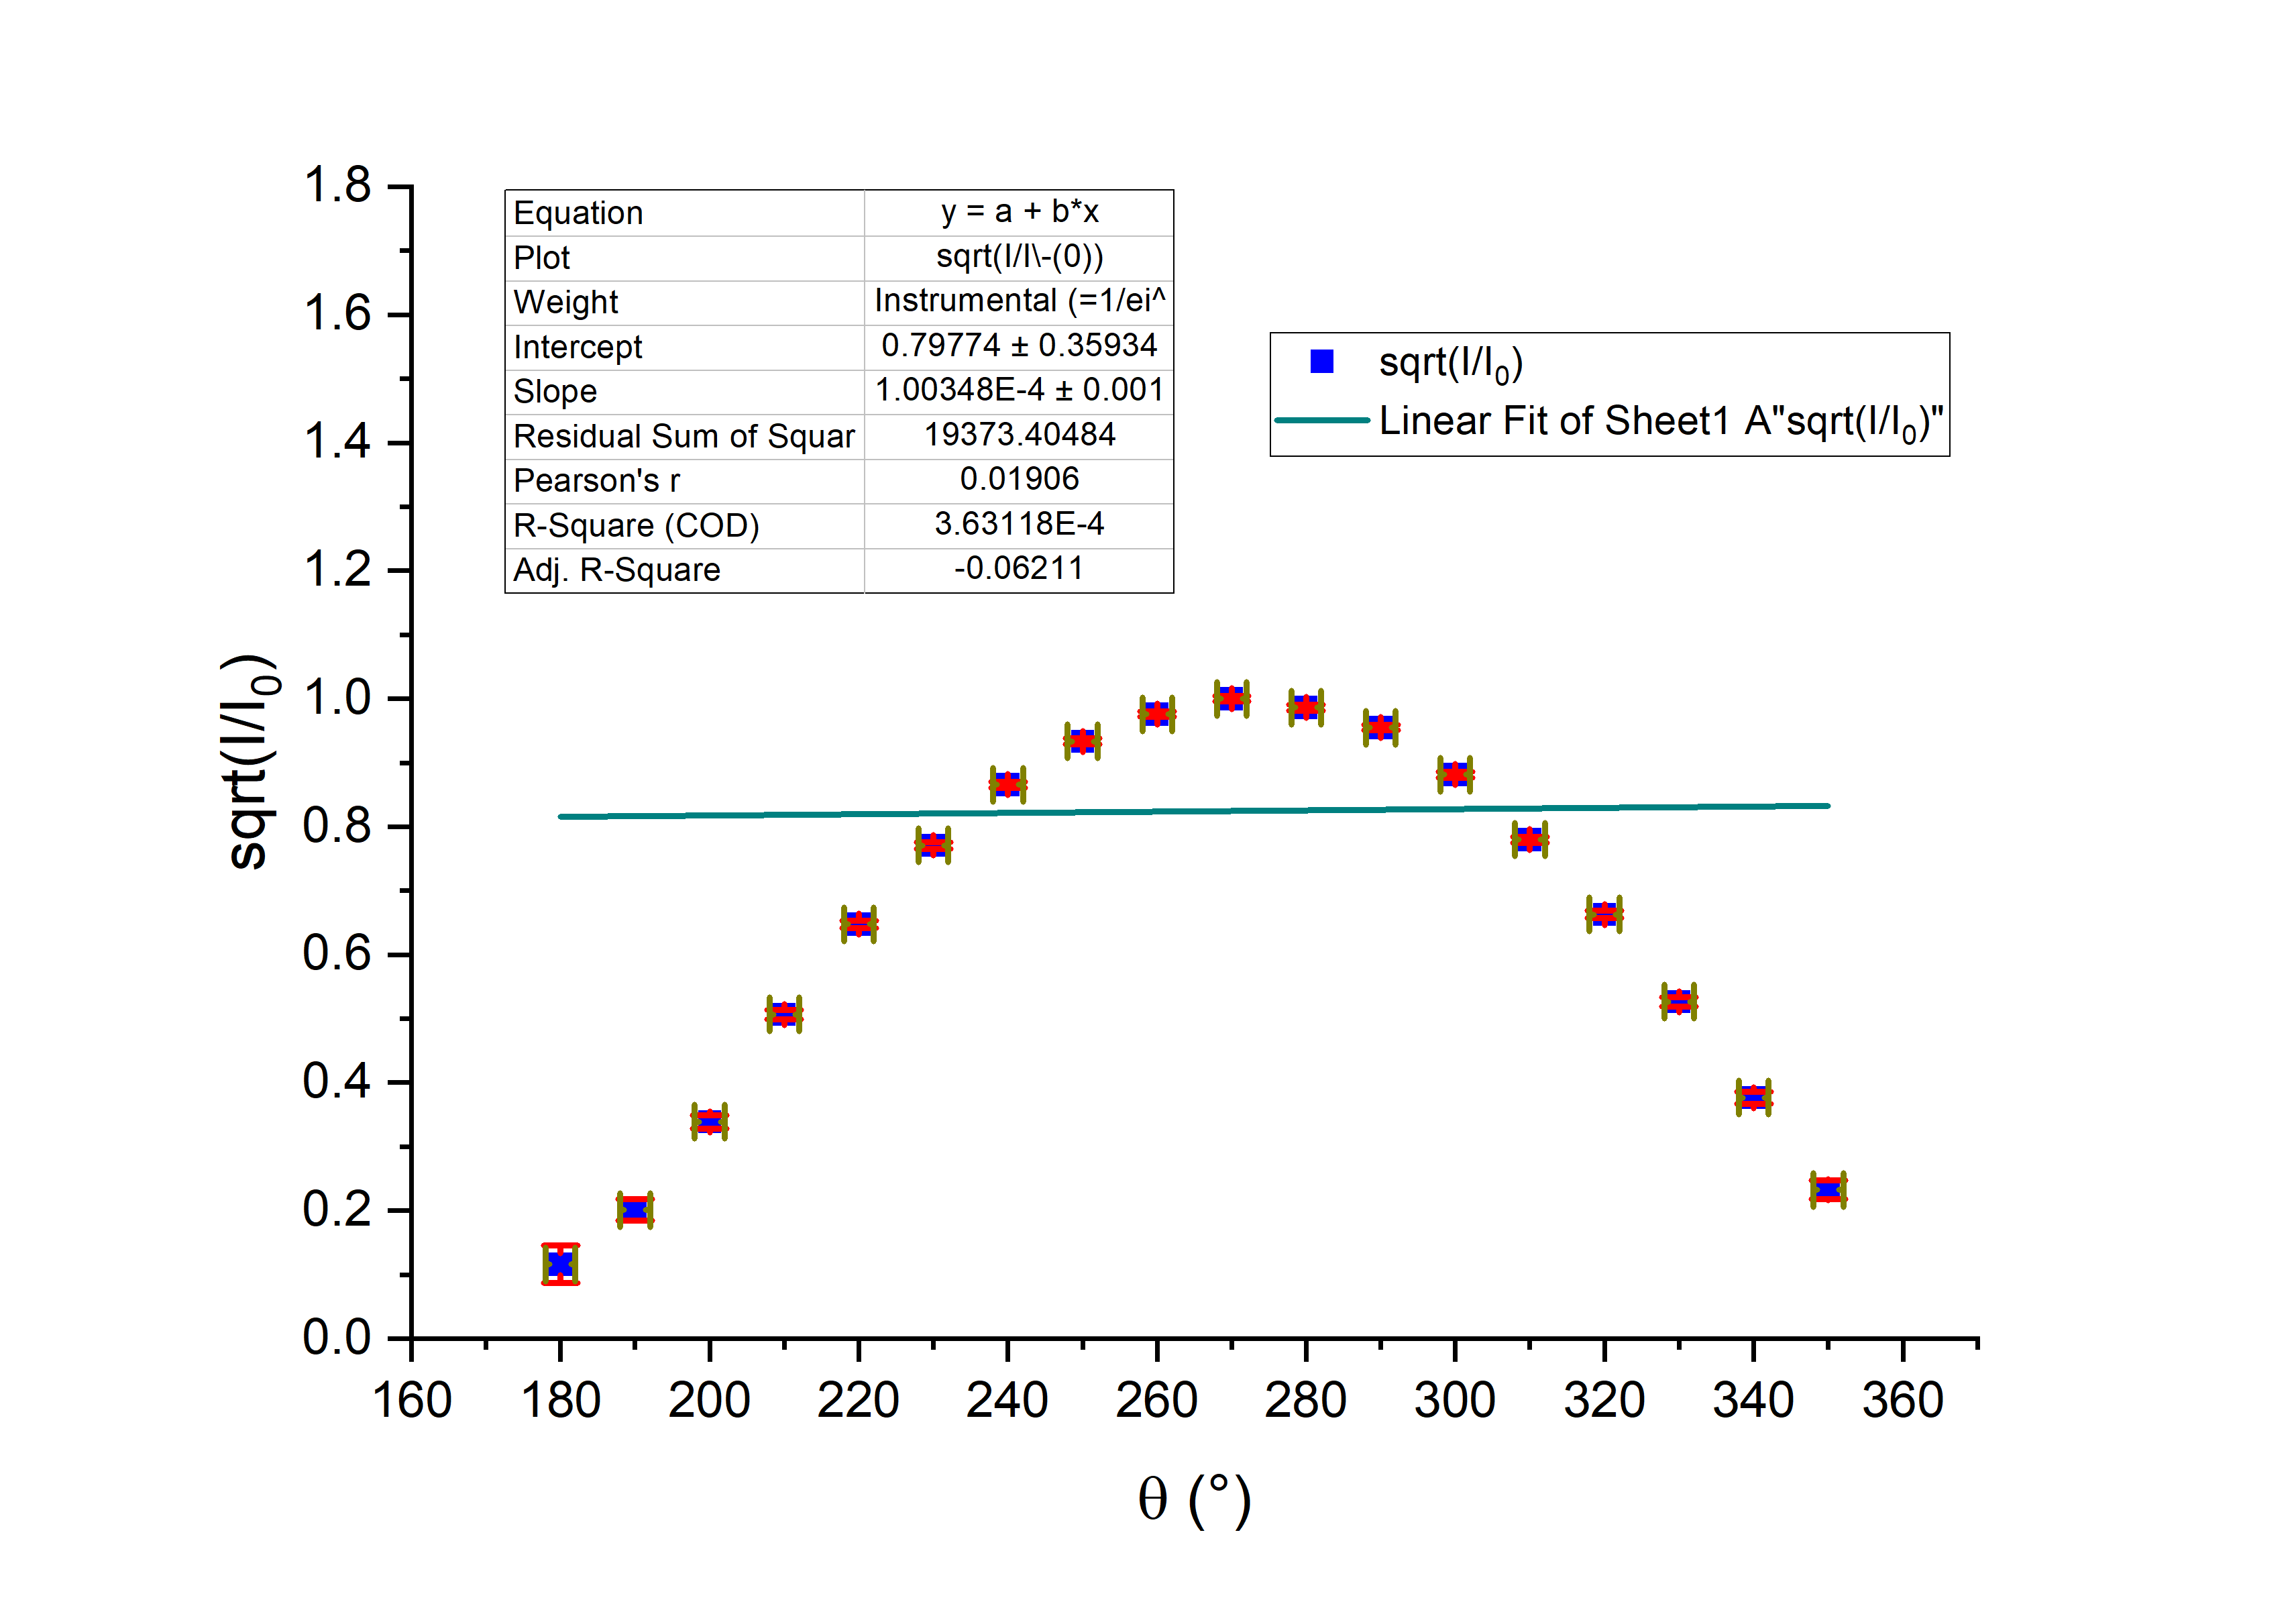
\includegraphics[width=0.45\textwidth]{C00.png}
    }\hspace{5mm}
	\caption{$\sqrt{I/I_0}$ vs. $\theta$ relation when rotation angle is 20$^\circ$.}
	\label{fig::0degree}
\end{figure}

\subsubsection{Rotation Angle: 20$^\circ$}

The measurement data for 20$^\circ$ rotation angle of 1/4-wave plate are shown in Table \ref{table::1/4,20}.  Note that when filling the data sheet, 0$^\circ$ and 90 $^\circ$ are mistaken and the mistake is corrected in the report.

\begin{table}[H]
	\centering
	\begin{tabular}{cc||cc}
		\multicolumn{4}{c}{Rotation angle of 1/4-wave plate: 20$^\circ$}                                                                                                                            \\
		\hline
		\multicolumn{2}{c}{Maximum Electric Current $I_0$} & \multicolumn{2}{c}{0.707 $\pm$ 0.001 [$\mu$A]}                                                                                         \\
		\hline
		$\theta\,\,[^\circ] \pm 2[^\circ]$                 & $I\,\,[\mu\text{A}] \pm 0.001\,\,[\mu\text{A}]$ & $\theta\,\,[^\circ] \pm 2[^\circ]$ & $I\,\,[\mu\text{A}] \pm 0.001\,\,[\mu\text{A}]$ \\
		\hline
		0                                                  & 0.31                                            & 180                                & 0.30                                            \\
		10                                                 & 0.21                                            & 190                                & 0.22                                            \\
		20                                                 & 0.19                                            & 200                                & 0.20                                            \\
		30                                                 & 0.24                                            & 210                                & 0.24                                            \\
		40                                                 & 0.36                                            & 220                                & 0.37                                            \\
		50                                                 & 0.51                                            & 230                                & 0.52                                            \\
		60                                                 & 0.70                                            & 240                                & 0.71                                            \\
		70                                                 & 0.89                                            & 250                                & 0.88                                            \\
		80                                                 & 1.05                                            & 260                                & 1.04                                            \\
		90                                                 & 1.20                                            & 270                                & 1.18                                            \\
		100                                                & 1.26                                            & 280                                & 1.27                                            \\
		110                                                & 1.26                                            & 290                                & 1.32                                            \\
		120                                                & 1.24                                            & 300                                & 1.28                                            \\
		130                                                & 1.16                                            & 310                                & 1.15                                            \\
		140                                                & 0.98                                            & 320                                & 0.98                                            \\
		150                                                & 0.80                                            & 330                                & 0.82                                            \\
		160                                                & 0.61                                            & 340                                & 0.63                                            \\
		170                                                & 0.45                                            & 350                                & 0.45                                            \\
		\hline
	\end{tabular}
	\caption{Measurement data for the 1/4-wave plate (rotation angle 20$^\circ$).}
	\label{table::1/4,20}
\end{table}

Similar to the previous section, $\sqrt{I/I_0}$ is calculated and the results are presented in Table \ref{TableSqrt20} (For sample calculation please refer to section \ref{sec:0degree}, which will not be repeated here).

\begin{table}[H]
	\centering
	\begin{tabular}{cc||cc}
		\hline
		$\theta\,\,[^\circ] \pm 2[^\circ]$ & $\sqrt{I/I_0}$       & $\theta\,\,[^\circ] \pm 2[^\circ]$ & $\sqrt{I/I_0}$      \\
		\hline
		0                                  & 0.485    $\pm$ 0.008 & 180                                & 0.477   $\pm$ 0.009 \\
		10                                 & 0.399    $\pm$ 0.010 & 190                                & 0.408   $\pm$ 0.010 \\
		20                                 & 0.379    $\pm$ 0.011 & 200                                & 0.389   $\pm$ 0.010 \\
		30                                 & 0.426    $\pm$ 0.009 & 210                                & 0.426   $\pm$ 0.009 \\
		40                                 & 0.522    $\pm$ 0.008 & 220                                & 0.529   $\pm$ 0.008 \\
		50                                 & 0.622    $\pm$ 0.007 & 230                                & 0.628   $\pm$ 0.007 \\
		60                                 & 0.728    $\pm$ 0.006 & 240                                & 0.733   $\pm$ 0.006 \\
		70                                 & 0.821    $\pm$ 0.006 & 250                                & 0.816   $\pm$ 0.006 \\
		80                                 & 0.892    $\pm$ 0.005 & 260                                & 0.888   $\pm$ 0.005 \\
		90                                 & 0.953    $\pm$ 0.005 & 270                                & 0.945   $\pm$ 0.005 \\
		100                                & 0.977    $\pm$ 0.005 & 280                                & 0.981   $\pm$ 0.005 \\
		110                                & 0.977    $\pm$ 0.005 & 290                                & 1.000   $\pm$ 0.005 \\
		120                                & 0.969    $\pm$ 0.005 & 300                                & 0.985   $\pm$ 0.005 \\
		130                                & 0.937    $\pm$ 0.005 & 310                                & 0.933   $\pm$ 0.005 \\
		140                                & 0.862    $\pm$ 0.005 & 320                                & 0.862   $\pm$ 0.005 \\
		150                                & 0.778    $\pm$ 0.006 & 330                                & 0.788   $\pm$ 0.006 \\
		160                                & 0.680    $\pm$ 0.006 & 340                                & 0.691   $\pm$ 0.006 \\
		170                                & 0.584    $\pm$ 0.007 & 350                                & 0.584   $\pm$ 0.007 \\
		\hline
	\end{tabular}
	\caption{Results for $\sqrt{I/I_0}$ when rotation angle is 20$^\circ$.}\label{TableSqrt20}
\end{table}

Then the relationship of $\sqrt{I/I_0}$ and $\theta$ are plotted in polar coordinate (Fig.\ref{fig::20degree}).

\begin{figure}[H]
	\centering
	\subfigure[$\sqrt{I/I_0}$ vs. $\theta$ relation in polar coordinate when rotation angle is 20$^\circ$.]{
    	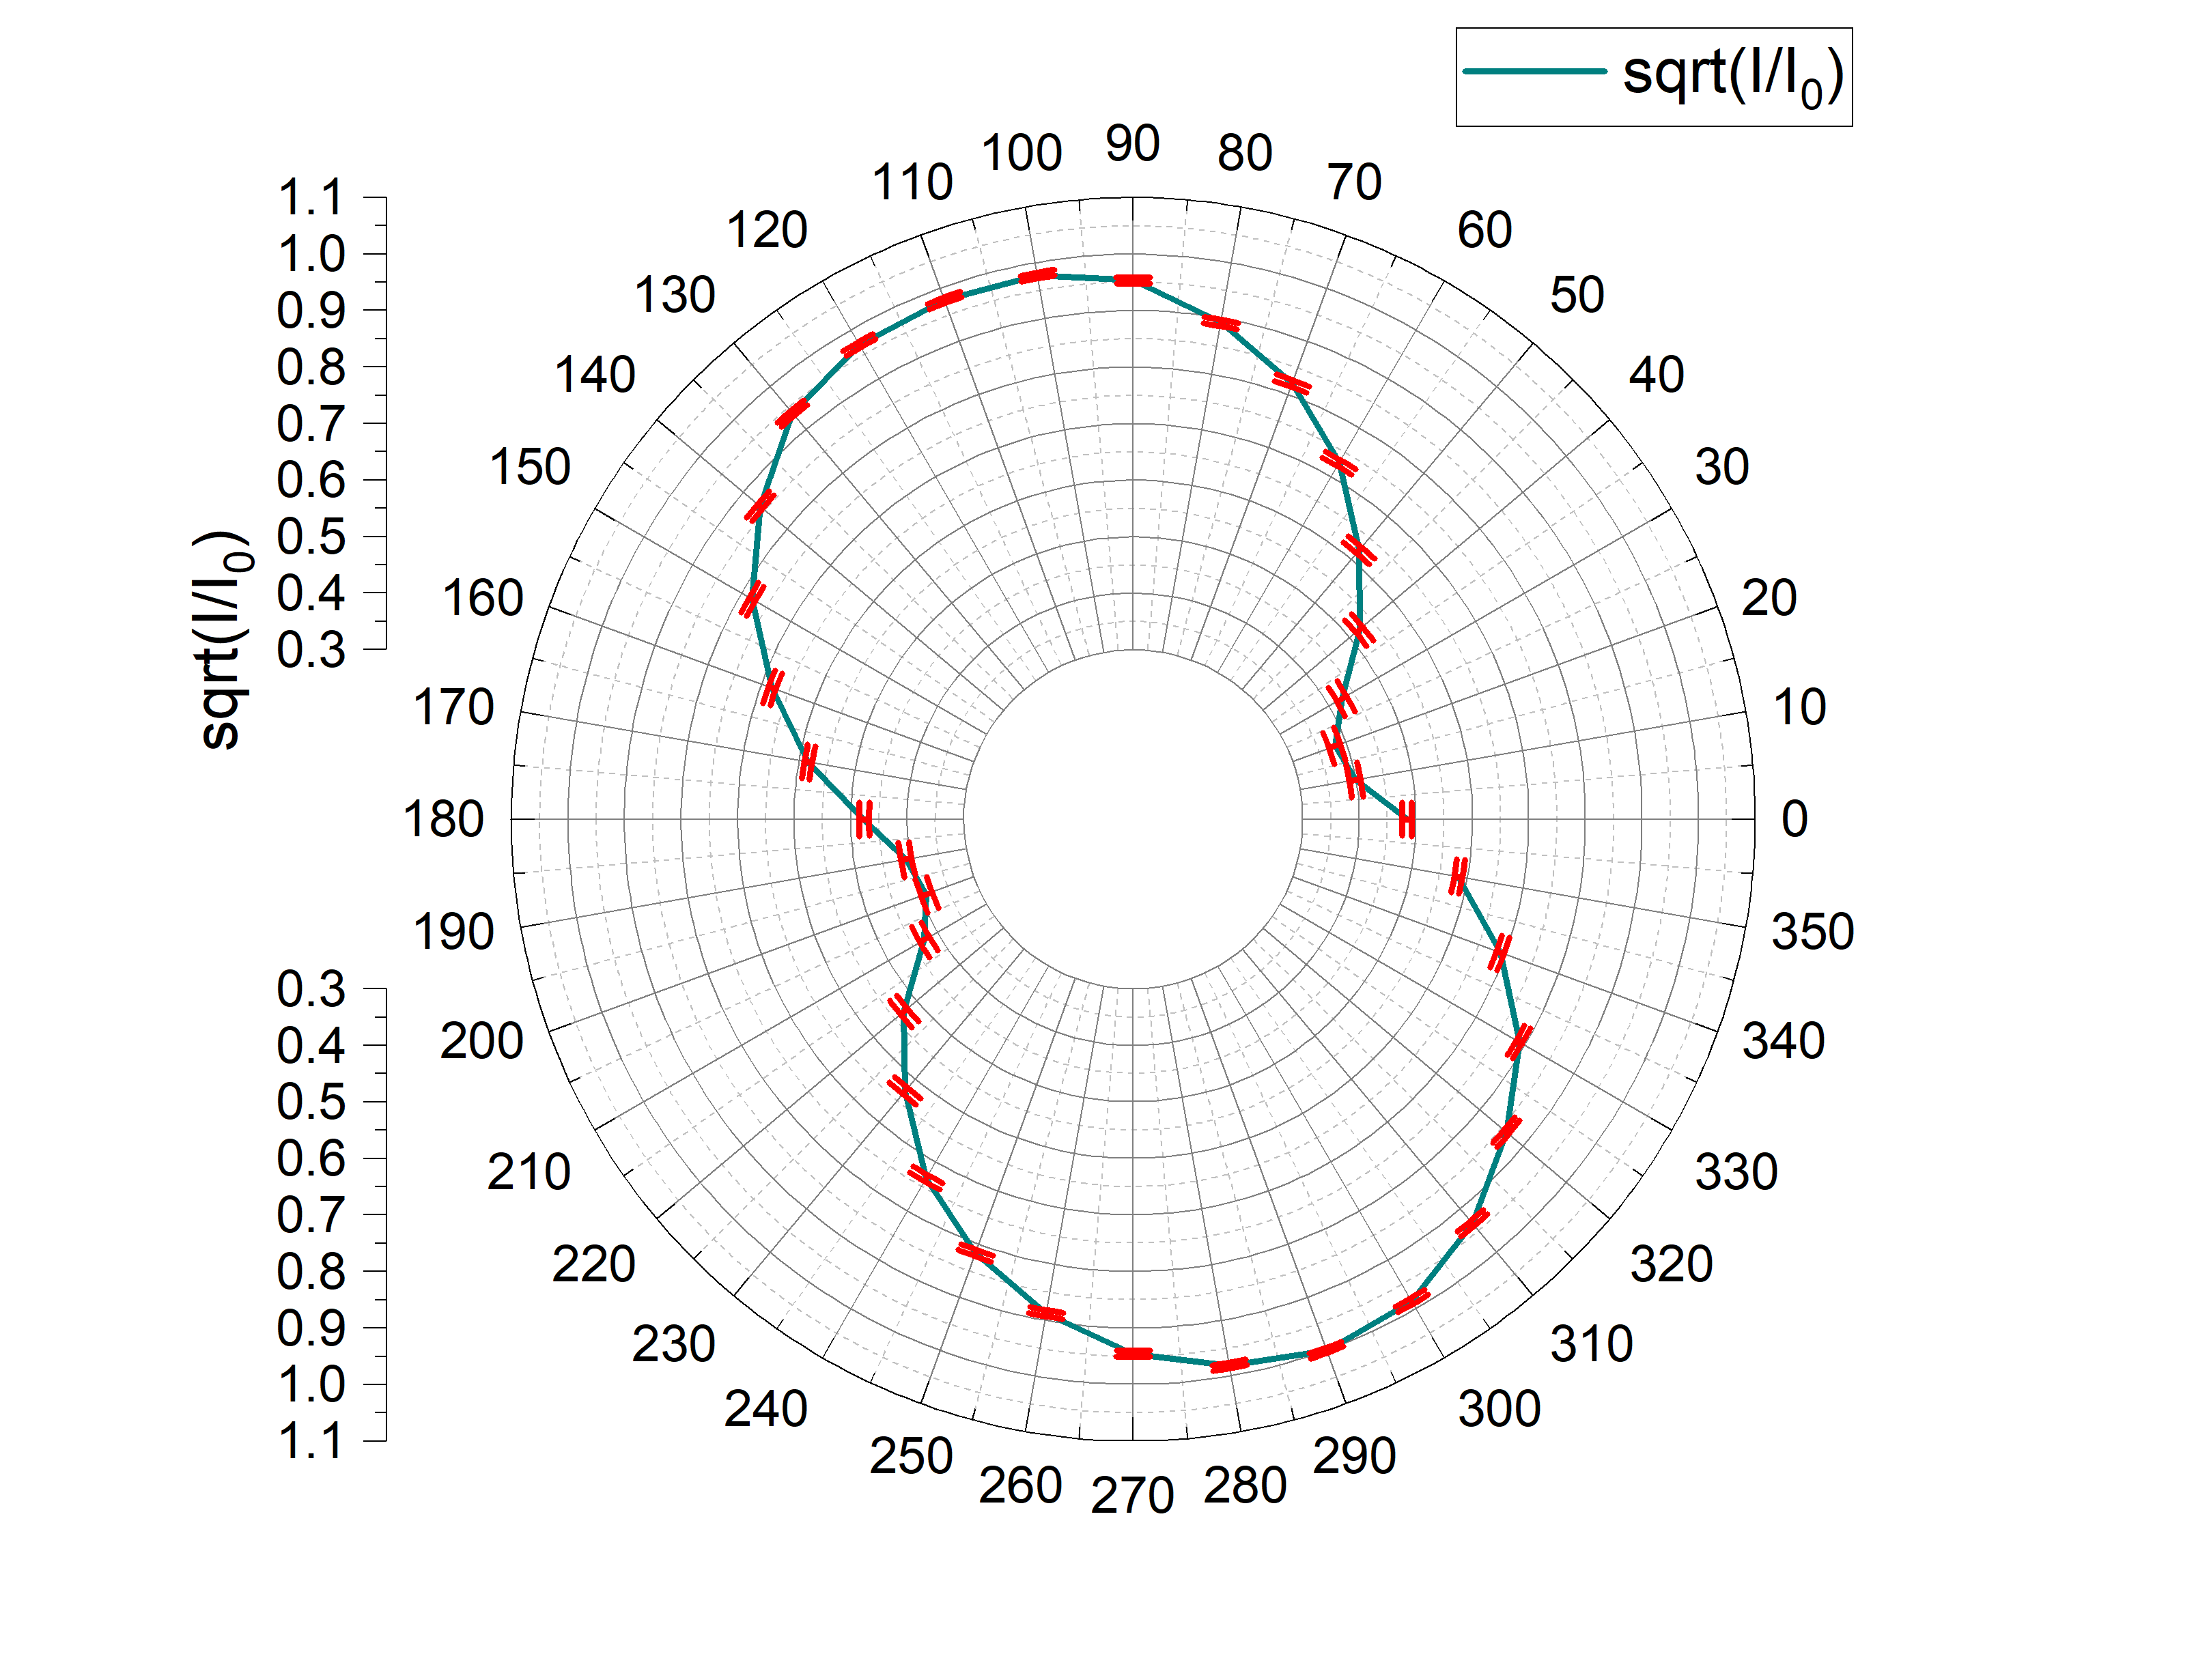
\includegraphics[width=0.45\textwidth]{20.png}
    }\hspace{5mm}
	\subfigure[$\sqrt{I/I_0}$ vs. $\theta$ relation in Cartesian coordinate when rotation angle is 20$^\circ$.]{
    	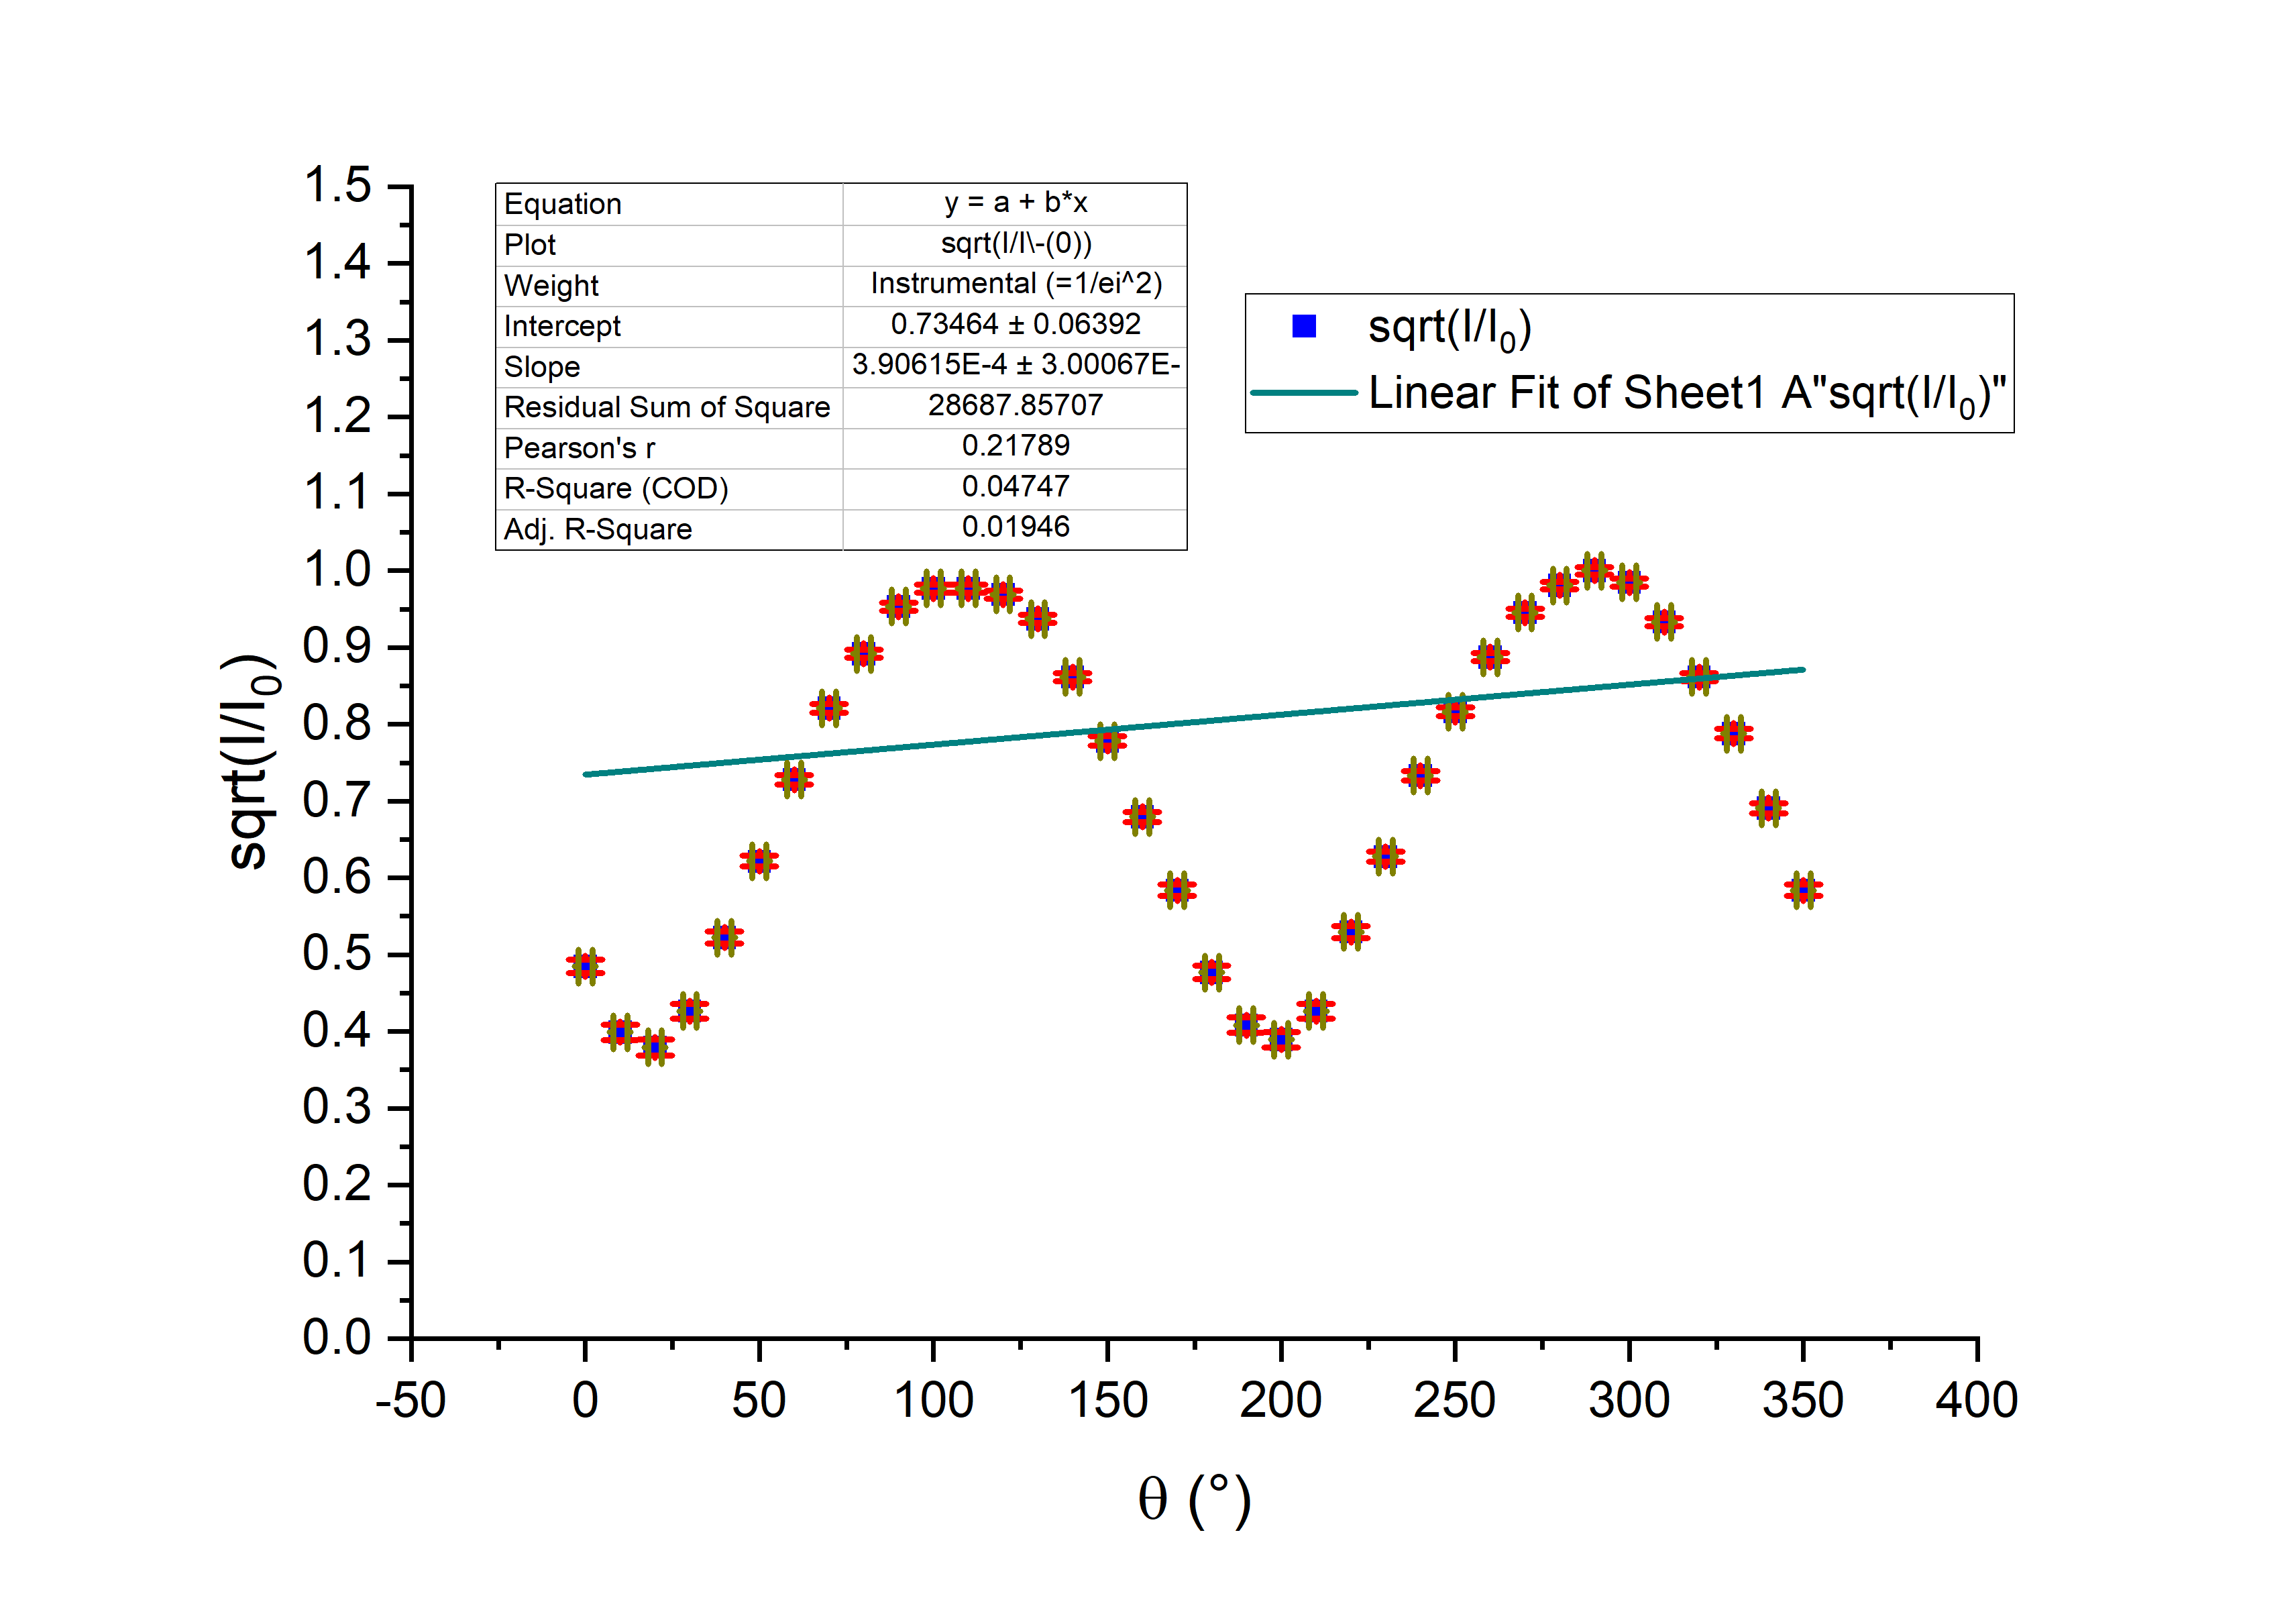
\includegraphics[width=0.45\textwidth]{C20.png}
    }\hspace{5mm}
	\caption{$\sqrt{I/I_0}$ vs. $\theta$ relation when rotation angle is 20$^\circ$.}
	\label{fig::20degree}
\end{figure}


\subsubsection{Rotation Angle: 45$^\circ$}

The measurement data for 45$^\circ$ rotation angle of 1/4-wave plate are shown in Table \ref{table::1/4,45}.  Note that when filling the data sheet, 0$^\circ$ and 90$^\circ$ are mistaken and the mistake is corrected in the report.

\begin{table}[H]
	\centering
	\begin{tabular}{cc||cc}
		\multicolumn{4}{c}{Rotation angle of 1/4-wave plate: 45$^\circ$}                                                                                                                            \\
		\hline
		\multicolumn{2}{c}{Maximum Electric Current $I_0$} & \multicolumn{2}{c}{0.395 $\pm$ 0.001 [$\mu$A]}                                                                                         \\
		\hline
		$\theta\,\,[^\circ] \pm 2[^\circ]$                 & $I\,\,[\mu\text{A}] \pm 0.001\,\,[\mu\text{A}]$ & $\theta\,\,[^\circ] \pm 2[^\circ]$ & $I\,\,[\mu\text{A}] \pm 0.001\,\,[\mu\text{A}]$ \\
		\hline
		0                                                  & 0.69                                            & 180                                & 0.70                                            \\
		10                                                 & 0.69                                            & 190                                & 0.71                                            \\
		20                                                 & 0.70                                            & 200                                & 0.73                                            \\
		30                                                 & 0.74                                            & 210                                & 0.74                                            \\
		40                                                 & 0.76                                            & 220                                & 0.77                                            \\
		50                                                 & 0.78                                            & 230                                & 0.79                                            \\
		60                                                 & 0.80                                            & 240                                & 0.80                                            \\
		70                                                 & 0.80                                            & 250                                & 0.81                                            \\
		80                                                 & 0.81                                            & 260                                & 0.81                                            \\
		90                                                 & 0.82                                            & 270                                & 0.81                                            \\
		100                                                & 0.79                                            & 280                                & 0.80                                            \\
		110                                                & 0.78                                            & 290                                & 0.80                                            \\
		120                                                & 0.77                                            & 300                                & 0.79                                            \\
		130                                                & 0.76                                            & 310                                & 0.76                                            \\
		140                                                & 0.74                                            & 320                                & 0.72                                            \\
		150                                                & 0.72                                            & 330                                & 0.71                                            \\
		160                                                & 0.71                                            & 340                                & 0.71                                            \\
		170                                                & 0.70                                            & 350                                & 0.70                                            \\
		\hline
	\end{tabular}
	\caption{Measurement data for the 1/4-wave plate (rotation angle 45$^\circ$).}
	\label{table::1/4,45}
\end{table}

Similar to the previous section, $\sqrt{I/I_0}$ is calculated and the results are presented in Table \ref{TableSqrt45} (For sample calculation please refer to section \ref{sec:0degree}, which will not be repeated here).

\begin{table}[H]
	\centering
	\begin{tabular}{cc||cc}
		\hline
		$\theta\,\,[^\circ] \pm 2[^\circ]$ & $\sqrt{I/I_0}$      & $\theta\,\,[^\circ] \pm 2[^\circ]$ & $\sqrt{I/I_0}$      \\
		\hline
		0                                  & 0.917   $\pm$ 0.009 & 180                                & 0.924   $\pm$ 0.009 \\
		10                                 & 0.917   $\pm$ 0.009 & 190                                & 0.931   $\pm$ 0.009 \\
		20                                 & 0.924   $\pm$ 0.009 & 200                                & 0.944   $\pm$ 0.009 \\
		30                                 & 0.950   $\pm$ 0.009 & 210                                & 0.950   $\pm$ 0.009 \\
		40                                 & 0.963   $\pm$ 0.009 & 220                                & 0.969   $\pm$ 0.009 \\
		50                                 & 0.975   $\pm$ 0.009 & 230                                & 0.982   $\pm$ 0.009 \\
		60                                 & 0.988   $\pm$ 0.009 & 240                                & 0.988   $\pm$ 0.009 \\
		70                                 & 0.988   $\pm$ 0.009 & 250                                & 0.994   $\pm$ 0.009 \\
		80                                 & 0.994   $\pm$ 0.009 & 260                                & 0.994   $\pm$ 0.009 \\
		90                                 & 1.000   $\pm$ 0.009 & 270                                & 0.994   $\pm$ 0.009 \\
		100                                & 0.982   $\pm$ 0.009 & 280                                & 0.988   $\pm$ 0.009 \\
		110                                & 0.975   $\pm$ 0.009 & 290                                & 0.988   $\pm$ 0.009 \\
		120                                & 0.969   $\pm$ 0.009 & 300                                & 0.982   $\pm$ 0.009 \\
		130                                & 0.963   $\pm$ 0.009 & 310                                & 0.963   $\pm$ 0.009 \\
		140                                & 0.950   $\pm$ 0.009 & 320                                & 0.937   $\pm$ 0.009 \\
		150                                & 0.937   $\pm$ 0.009 & 330                                & 0.931   $\pm$ 0.009 \\
		160                                & 0.931   $\pm$ 0.009 & 340                                & 0.931   $\pm$ 0.009 \\
		170                                & 0.924   $\pm$ 0.009 & 350                                & 0.924   $\pm$ 0.009 \\
		\hline
	\end{tabular}
	\caption{Results for $\sqrt{I/I_0}$ when rotation angle is 45$^\circ$.}\label{TableSqrt45}
\end{table}

Then the relationship of $\sqrt{I/I_0}$ and $\theta$ are plotted in polar coordinate (Figure \ref{fig::45degree}).

\begin{figure}[H]
	\centering
	\subfigure[$\sqrt{I/I_0}$ vs. $\theta$ relation in polar coordinate when rotation angle is 45$^\circ$.]{
    	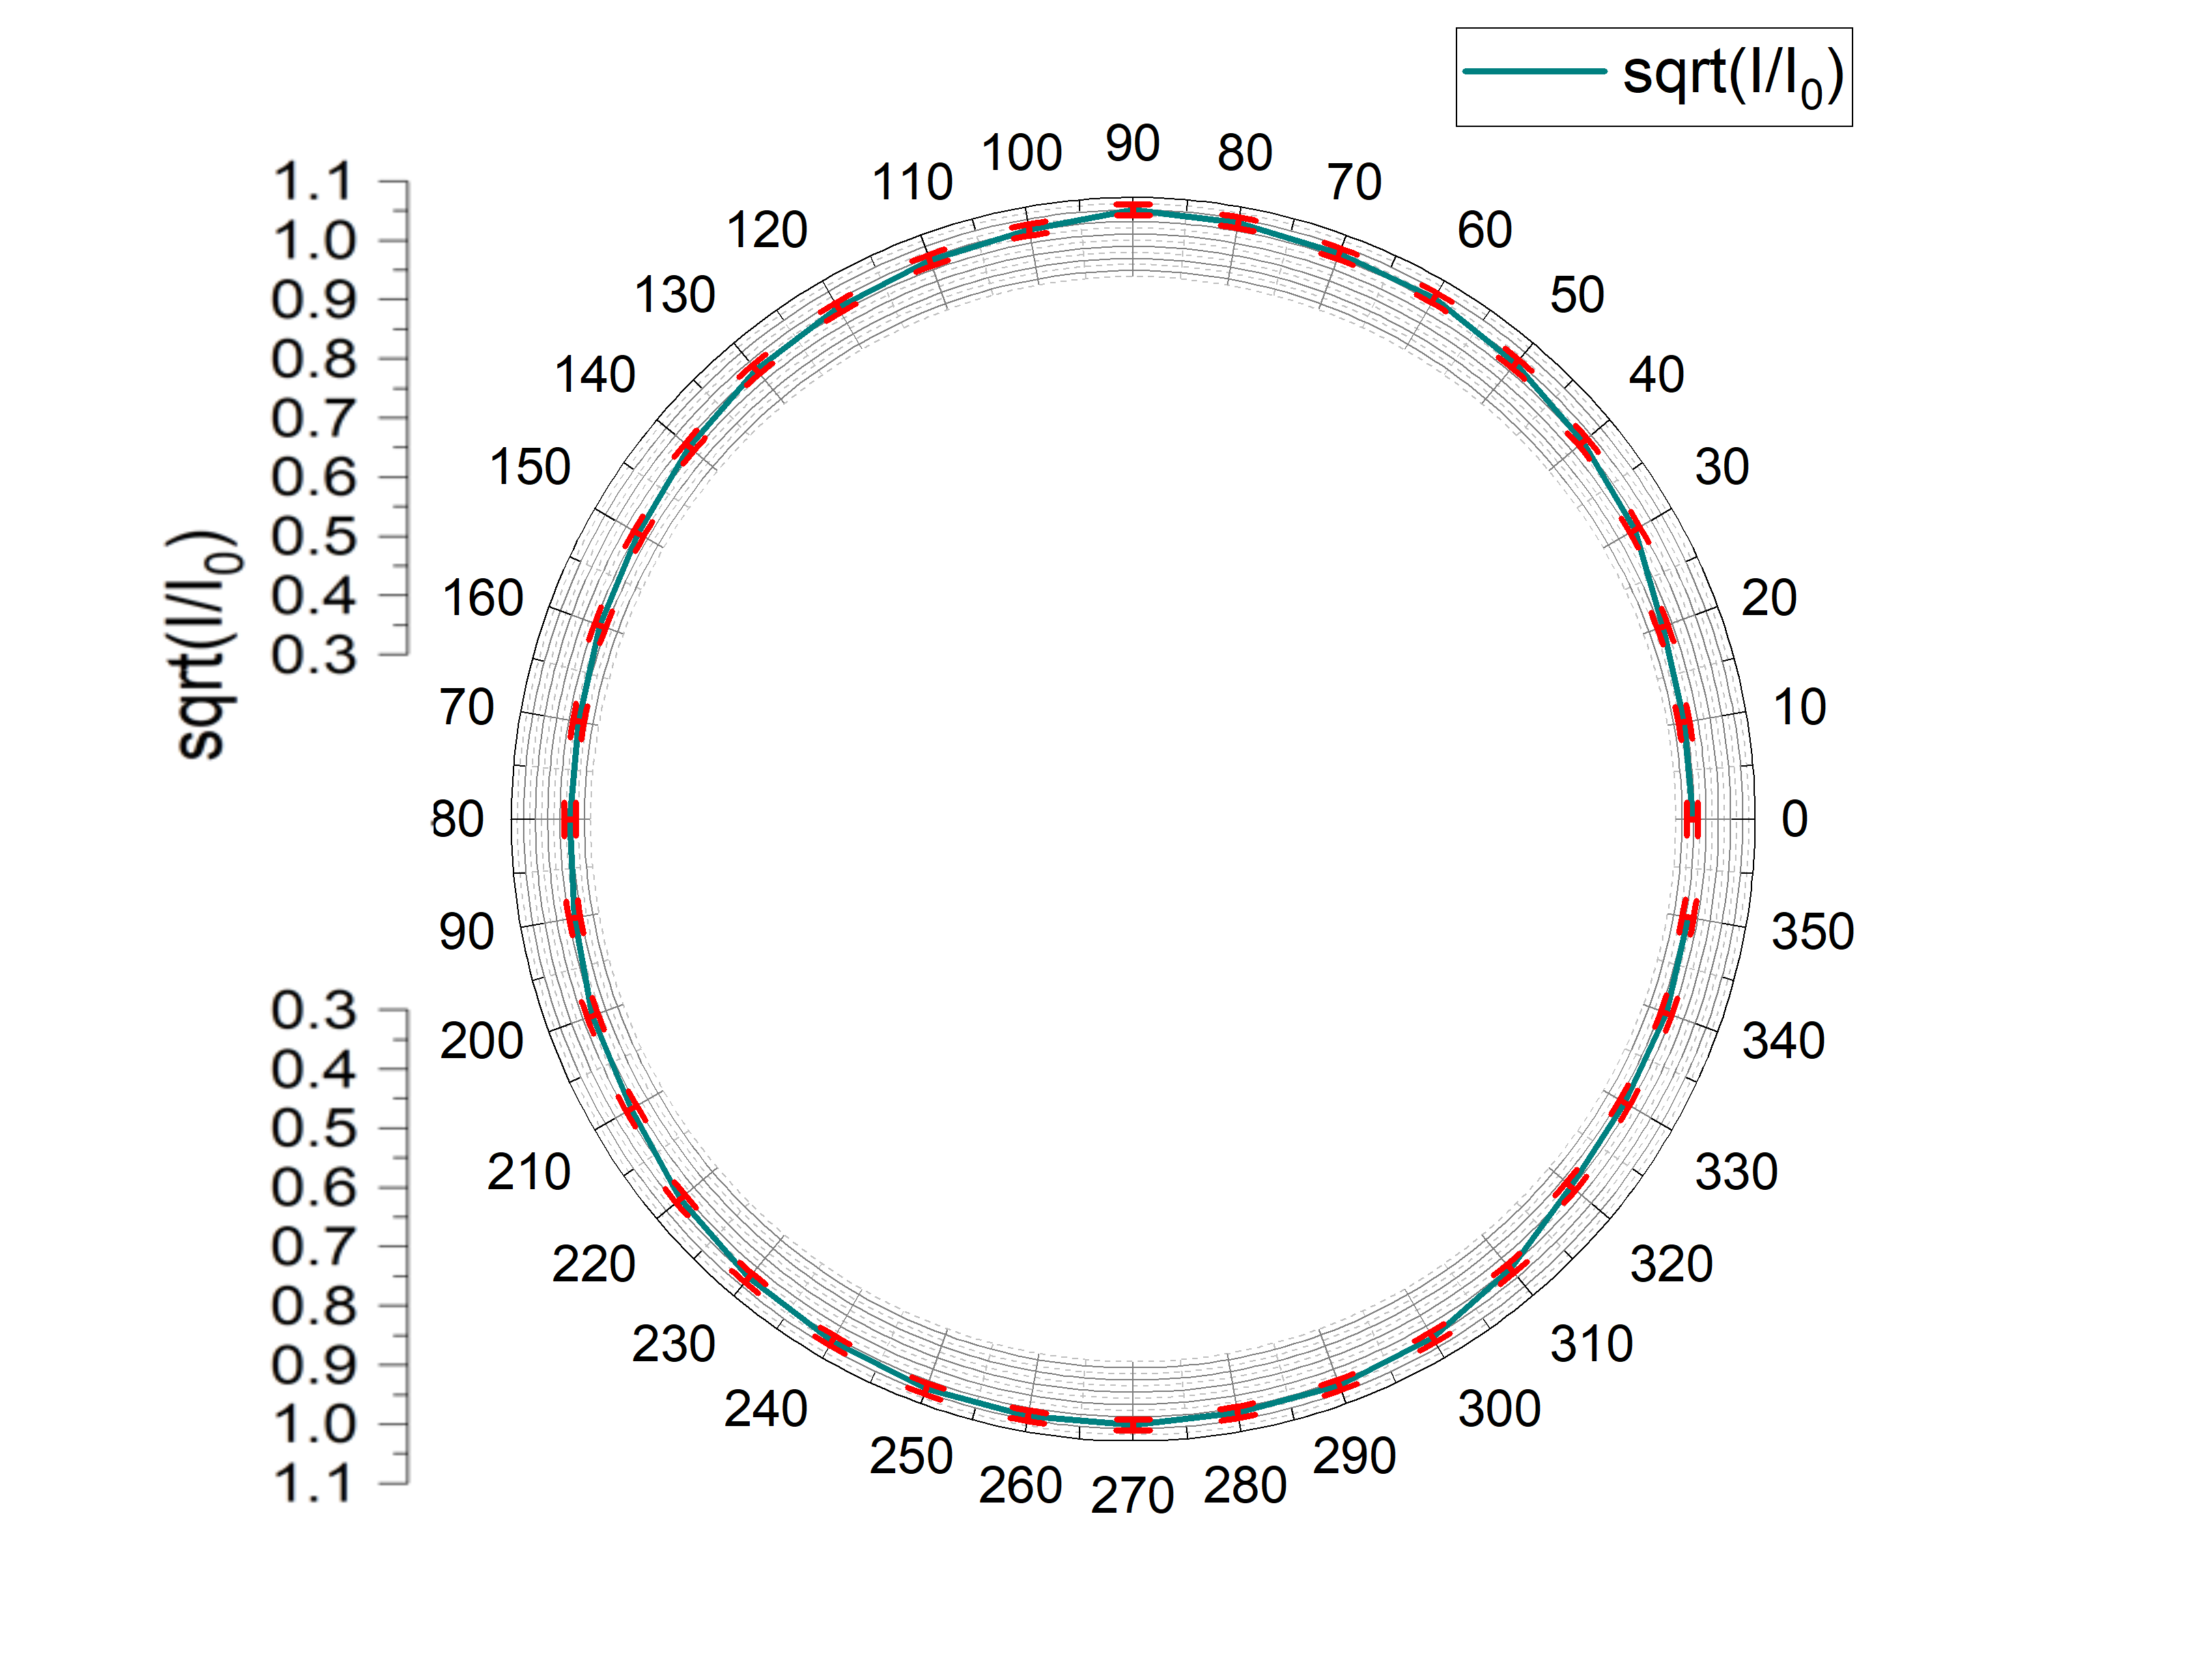
\includegraphics[width=0.45\textwidth]{45.png}
    }\hspace{5mm}
	\subfigure[$\sqrt{I/I_0}$ vs. $\theta$ relation in Cartesian coordinate when rotation angle is 45$^\circ$.]{
    	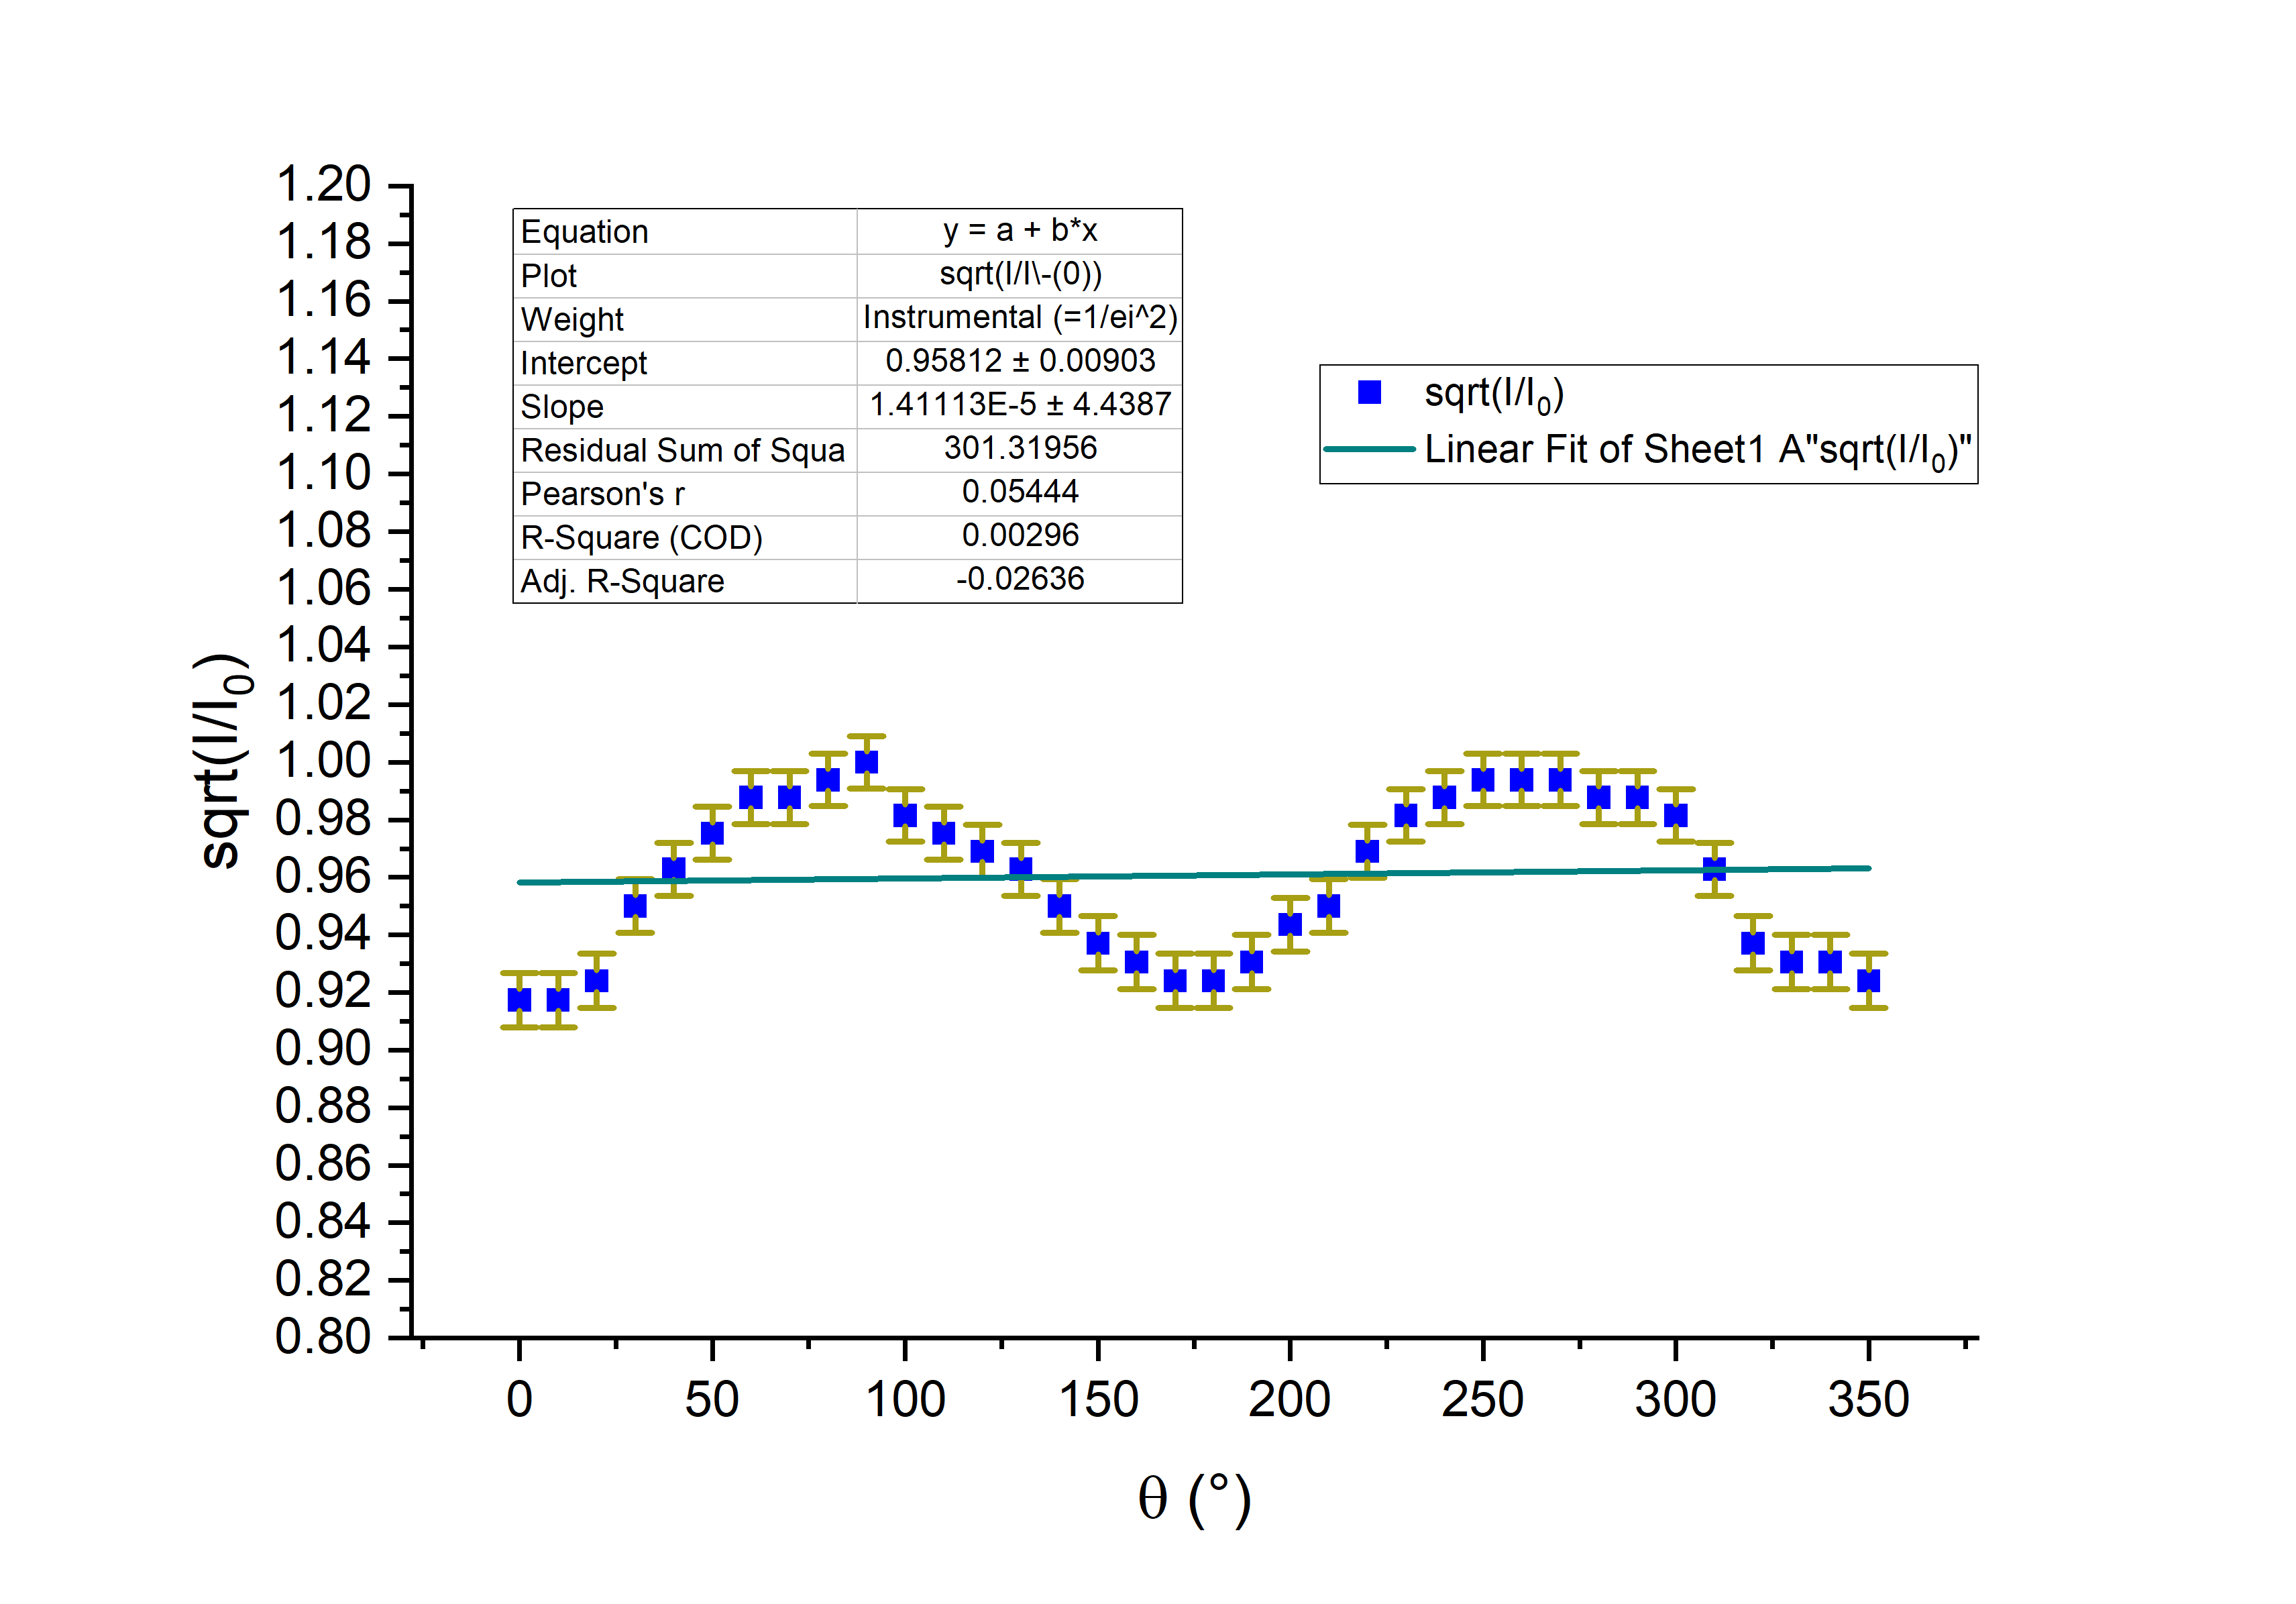
\includegraphics[width=0.45\textwidth]{C45.png}
    }\hspace{5mm}
	\caption{$\sqrt{I/I_0}$ vs. $\theta$ relation when rotation angle is 45$^\circ$.}
	\label{fig::45degree}
\end{figure}

To compare the result with circular polarization, as described in the procedure part, the data is also plotted in Cartesian coordinate and linear fit is performed (Fig.\ref{fig::45degree}(b)). The slope of the linear fitting is $1.4 \times 10^{-5}$.






\section{Uncertainty Analysis}

\subsection{Uncertainty for Data in Demonstration of Malus' Law}

The uncertainty of $\cos^2\theta$ is
\begin{align*}
	u_{\cos^{2}\theta} & =\sqrt{(\frac{\partial \cos^{2}\theta}{\partial \theta}u_{\theta})^{2}} \\
	                   & =|-2\cos\theta\sin\theta u_{\theta}|                                    \\
	                   & =|\sin2\theta u_{\theta}|,
\end{align*}
where $u_\theta = 2[^\circ] = \pi/90$. Take $\theta$ = 5$^\circ$ as an example,
$$u_{\cos^{2}\theta}=|\sin2\theta u_{\theta}|=|\sin({2\times 5^\circ})\times \frac{\pi}{90}|=0.006,$$
All the results are shown in Table \ref{table::uncosine}.\\

The uncertainty of $I/I_0$ is
\begin{align*}
	u_{I/I_{0}} & =\sqrt{(\frac{\partial I/I_0}{\partial I}u_{I})^{2}+(\frac{\partial I/I_0}{\partial I_{0}}u_{I_{0}})^{2}} \\
	            & =\sqrt{(\frac{u_{I}}{I_{0}})^{2}+(-\frac{I}{I_{0}^{2}}u_{I_{0}})^{2}},
\end{align*}
where $u_I = u_{I_0} = 0.01\,\,[\mu\text{A}]$, $I_0 = 2.21 \pm 0.01\,\,[\mu\text{A}]$. Take the second set of data as an example,
$$u_{I/I_{0}}= \sqrt{(\frac{u_{I}}{I_{0}})^{2}+(-\frac{I}{I_{0}^{2}}u_{I_{0}})^{2}}=\sqrt{(\frac{0.01}{2.21})^{2}+(-\frac{2.20}{2.21^{2}}\times 0.01)^{2}}=0.011,$$
All the results are shown in Table \ref{table::uncosine}.

\begin{table}[H]
	\centering
	\begin{tabular}{cc||cc}
		\hline
		$u_{\cos^2\theta}$ & $u_{I/I_0}$ & $u_{\cos^2\theta}$ & $u_{I/I_0}$ \\
		\hline
		0                  & 0.011       & 0.03               & 0.006       \\
		0.006              & 0.011       & 0.03               & 0.006       \\
		0.012              & 0.011       & 0.03               & 0.005       \\
		0.02               & 0.010       & 0.03               & 0.005       \\
		0.02               & 0.010       & 0.02               & 0.005       \\
		0.03               & 0.010       & 0.02               & 0.005       \\
		0.03               & 0.009       & 0.012              & 0.005       \\
		0.03               & 0.008       & 0.006              & 0.005       \\
		0.03               & 0.008       & 0                  & 0.005       \\
		0.03               & 0.007       &                    &             \\
		\hline
	\end{tabular}
	\caption{Uncertainty of $\cos^2\theta$ and $I/I_0$.}
	\label{table::uncosine}
\end{table}

\subsection{Uncertainty for Linearly Polarized Light and the Half-wave Plate}

In this part, the uncertainty of the measurement depends on the device, which is
$$u_\theta = 2^\circ.$$

\subsection{Uncertainty for Circularly and Elliptically Polarized Light and the 1/4-wave Plate}

The uncertainty of $\sqrt{I/I_0}$ is
\begin{align*}
	u_{\sqrt{I/I_{0}}} & =\sqrt{(\frac{\partial\sqrt{I/I_0}}{\partial I}u_{I})^{2}+(\frac{\partial\sqrt{I/I_0}}{\partial I_{0}}u_{I_{0}})^{2}} \\
	                   & =\sqrt{\frac{1}{4II_0}u_I^2+\frac{I}{4I_0^3}u_{I_0}^2},
\end{align*}
where $u_I = u_{I_0} = 0.01\,\,[\mu\text{A}]$, $I_0 = 1.48 \pm 0.01\,\,[\mu\text{A}]$ for rotation angle of 0$^\circ$, $I_0 = 1.32 \pm 0.01\,\,[\mu\text{A}]$ for rotation angle of 20$^\circ$, $I_0 = 0.82 \pm 0.01\,\,[\mu\text{A}]$ for rotation angle of 45$^\circ$. Take the first set of data as an example,
$$u_{\sqrt{I/I_{0}}}=\sqrt{\frac{1}{4\times 0.02 \times 1.48} \times 0.01^2+\frac{0.02}{4\times 1.48^3}\times 0.01^2}=0.03.$$
All the results are shown in Table \ref{TableUnc1/4}.

\begin{table}[H]
	\centering
	\begin{tabular}{ccc}
		\hline
		Rotation angle: $0^\circ$ & Rotation angle: $20^\circ$ & Rotation angle: $45^\circ$ \\
		$u_{\sqrt{I/I_{0}}}$      & $u_{\sqrt{I/I_{0}}}$       & $u_{\sqrt{I/I_{0}}}$       \\
		\hline
		0.03                      & 0.008                      & 0.009                      \\
		0.02                      & 0.010                      & 0.009                      \\
		0.010                     & 0.011                      & 0.009                      \\
		0.007                     & 0.009                      & 0.009                      \\
		0.006                     & 0.008                      & 0.009                      \\
		0.005                     & 0.007                      & 0.009                      \\
		0.005                     & 0.006                      & 0.009                      \\
		0.005                     & 0.006                      & 0.009                      \\
		0.004                     & 0.005                      & 0.009                      \\
		0.004                     & 0.005                      & 0.009                      \\
		0.004                     & 0.005                      & 0.009                      \\
		0.005                     & 0.005                      & 0.009                      \\
		0.005                     & 0.005                      & 0.009                      \\
		0.005                     & 0.005                      & 0.009                      \\
		0.006                     & 0.005                      & 0.009                      \\
		0.007                     & 0.006                      & 0.009                      \\
		0.010                     & 0.006                      & 0.009                      \\
		0.02                      & 0.007                      & 0.009                      \\
		0.03                      & 0.009                      & 0.009                      \\
		0.02                      & 0.010                      & 0.009                      \\
		0.010                     & 0.010                      & 0.009                      \\
		0.007                     & 0.009                      & 0.009                      \\
		0.006                     & 0.008                      & 0.009                      \\
		0.005                     & 0.007                      & 0.009                      \\
		0.005                     & 0.006                      & 0.009                      \\
		0.005                     & 0.006                      & 0.009                      \\
		0.004                     & 0.005                      & 0.009                      \\
		0.004                     & 0.005                      & 0.009                      \\
		0.004                     & 0.005                      & 0.009                      \\
		0.004                     & 0.005                      & 0.009                      \\
		0.005                     & 0.005                      & 0.009                      \\
		0.005                     & 0.005                      & 0.009                      \\
		0.006                     & 0.005                      & 0.009                      \\
		0.007                     & 0.006                      & 0.009                      \\
		0.009                     & 0.006                      & 0.009                      \\
		0.015                     & 0.007                      & 0.009                      \\
		\hline
	\end{tabular}
	\caption{Uncertainty for $\sqrt{I/I_0}$ when the rotation angle is $0^\circ$, $20^\circ$ and $45^\circ$.}\label{TableUnc1/4}
\end{table}



\section{Conclusion and Discussion}

\subsection{Conclusion}

\subsection{Demonstration of Malus' Law}

The slope of the fitting is 1.009 $\pm$ 0.004 and the Pearson's r is 0.9999, which is very close to 1. This suggests that the value of $I/I_0$ is proportional to the value of $\cos^2\theta$ with the coefficient to be about 1. 
Theoretically, by Eq. (\ref{eq::Malus’ law}), the slope is
$$\frac{I/I_0}{\cos^2\theta} = 1,$$
Therefore, the relative error is
$$\varepsilon = \frac{1.009-1}{1} \times 100\% = 0.9\%.$$
This in an acceptable range of error verifies the Malus' Law.

\subsection{Linearly Polarized Light and the Half-wave Plate}

The slope of the linear fit is $1.992 \pm 0.016$. Theoretically, as introduced in the Introduction part, the rotation angle of the polarization axis is twice of the origin angle for a half-wave plate. 
Therefore the theoretical value of the slope of our linear fitting is 2. The relative error is therefore
$$\varepsilon = \frac{1.992-2}{2}\times 100\% = -0.4\%.$$ 
This conforms to the theoretical fact.

\subsection{Circularly and Elliptically Polarized Light and the 1/4-wave Plate}

Here we conclude several points in this exercise.

\begin{itemize}
	\item From Table \ref{table::1/4,0} and Figure \ref{fig::0degree}, it can be seen that the maximum of light intensity occurs at about $\theta = 0^\circ$. This suggests that polarizing axis is parallel to the optical axis of the plate, which is the theoretical conclusion stated in the Introduction part. The shape of the plot also indicates that it is linearly polarized.
	\item From Table \ref{table::1/4,20} and Figure \ref{fig::20degree}, it can be seen that the maximum of light intensity occurs at about $\theta = 20^\circ$. This suggests that polarizing axis forms $20^\circ$ to the optical axis of the plate, which conforms to the fact stated in [4]. The shape of the plot also indicates that it is elliptically polarized.
	\item From Figure \ref{fig::45degree}, it can be seen that the value of $\sqrt{I/I_0}$ changes little when $\theta$ changes. Besides, the slop of linear fit of the plot of $\sqrt{I/I_0}$ vs. $\theta$ in the Cartesian coordinate in Figure \ref{fig::45degree} is $1.4 \times 10^{-5}$ but the Pearson's coefficient is only 0.0544. All the results suggest that $\sqrt{I/I_0}$ is a constant, with no relation with the value of $\theta$. Therefore it can be concluded that when rotation angle is 45$^\circ$, the light is circularly polarized. This conforms to the fact stated in the Introduction part.

\end{itemize}

Detailed analysis and discussion about experimental results are left to DISCUSSION part.

\subsection{Discussion}

Here we will discuss the problems in this exercise, some potential errors which may lead to huge variation, and some suggestions.

\subsubsection{Problems}

\begin{itemize}
	\item \textbf{Photocurrent:} Photocurrent meter reading varies continuously during experiments, which may cause huge errors.
	\item \textbf{Apparatus:} Photocurrent meter reading does not change significantly even if the rotation angle reaches 10$^\circ$ or 20$^\circ$.
	\item \textbf{Light path:} The apparatus may not be exactly horizontal, which may affect the ligh absorption.
\end{itemize}

\subsubsection{Potential errors}

\begin{itemize}
	\item Huge reading errors due to variation of photocurrent meter.
	\item Inaccurate measurement due to not sensitive apparatus at the boundary point.
	\item Constant variation due to non-horizontal light path.
\end{itemize}

\subsubsection{Imporvements}

\begin{itemize}
	\item Measure the data for more times and record the mean value of them.
	\item Apply more advanced experimental device, which can adjust the incident angle more flexible and precise$^{[6]}$.
	\item Adjust the apparatus and make sure it is properly set before conducting the experiment.
	\item Add one more polarizer into the apparatus$^{[5]}$.
\end{itemize}



\newpage
\section{Reference}
\noindent [1] Shipman, James; Wilson, Jerry D.; Higgins, Charles A. (2015). \textit{An Introduction to Physical Science, 14th Ed.} Cengage Learning. p. 187. ISBN 978-1-305-54467-3. \\
\noindent [2] Wolf, Mark J. P. (2008). \textit{The Video Game Explosion: A History from PONG to Playstation and Beyond.} ABC-CLIO. p. 315. ISBN 978-0313338687.
\noindent [3] M. Krzyzosiak (2021). Exercise 4 - lab manual [rev 2.8]. (UMJI-SJTU, Shanghai). \\
\noindent [4] University Physics, Section 33.5, Young and Freedman. \\ 
\noindent [5] DOI:\url{10.14139 /j.cnki.cn22-1228.2019.05.013}


\newpage
\section*{APPENDIX - DATA SHEET}

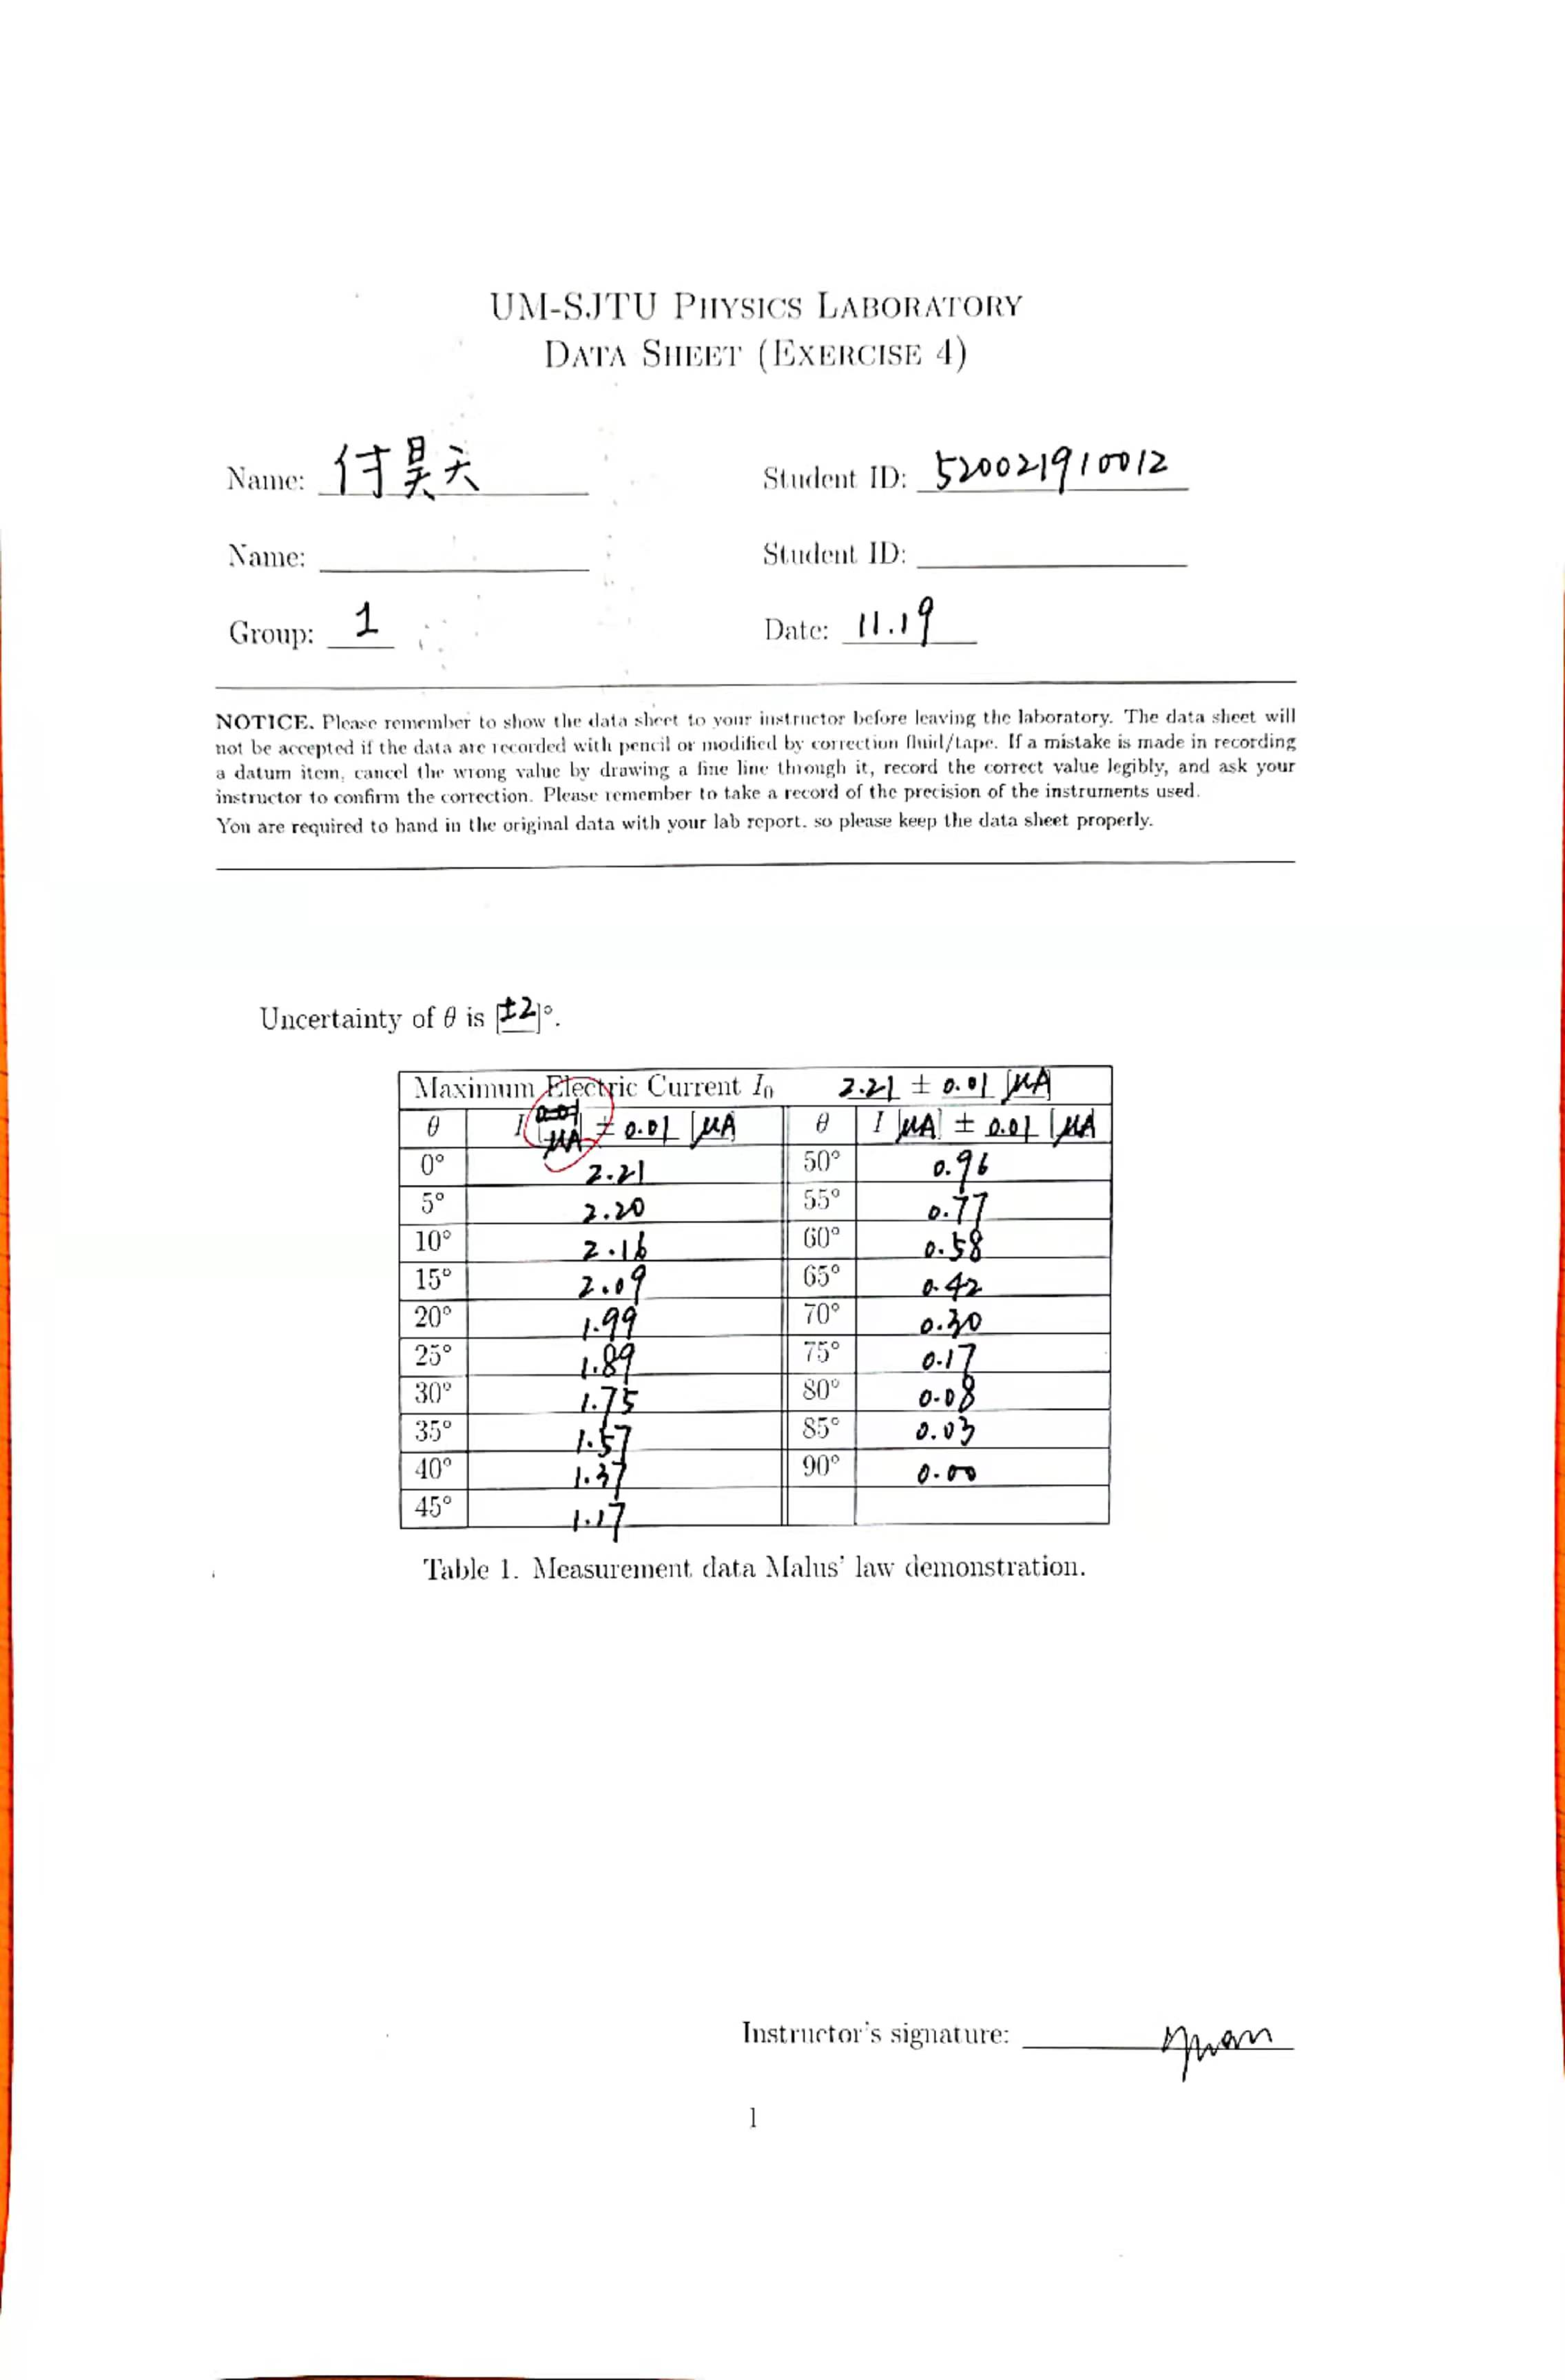
\includepdf{data_sheet1.pdf}
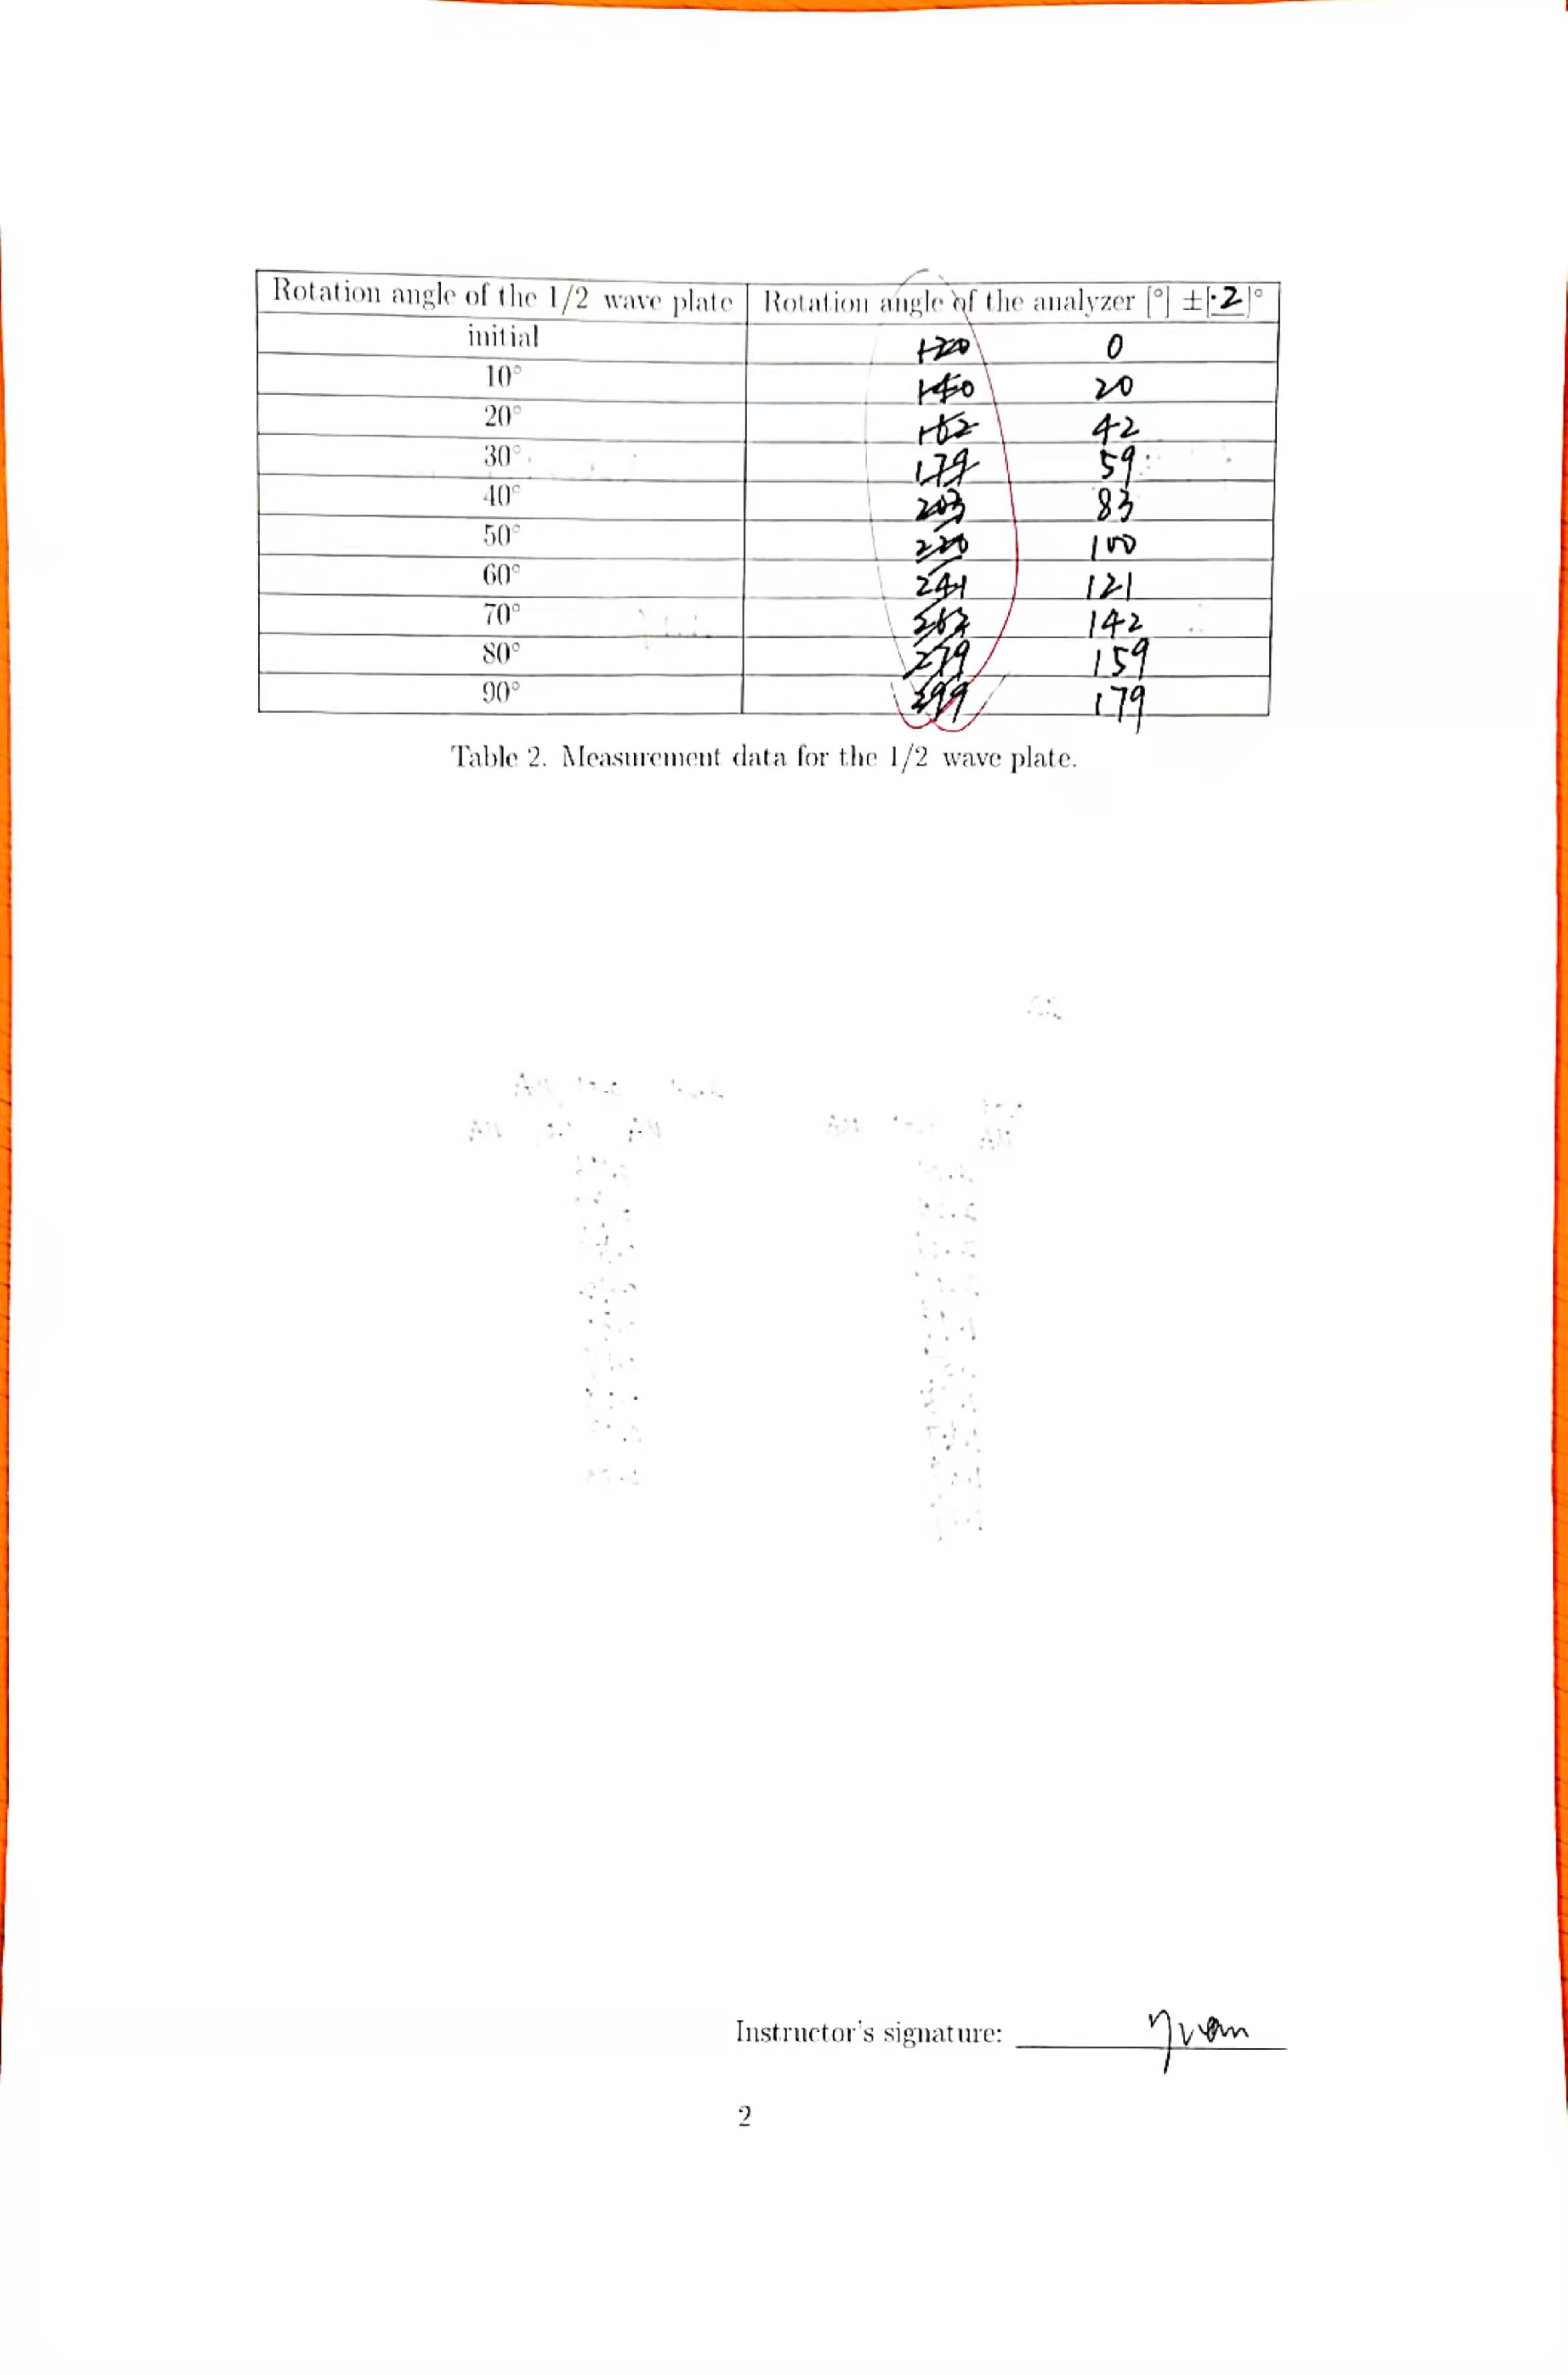
\includepdf{data_sheet2.pdf}
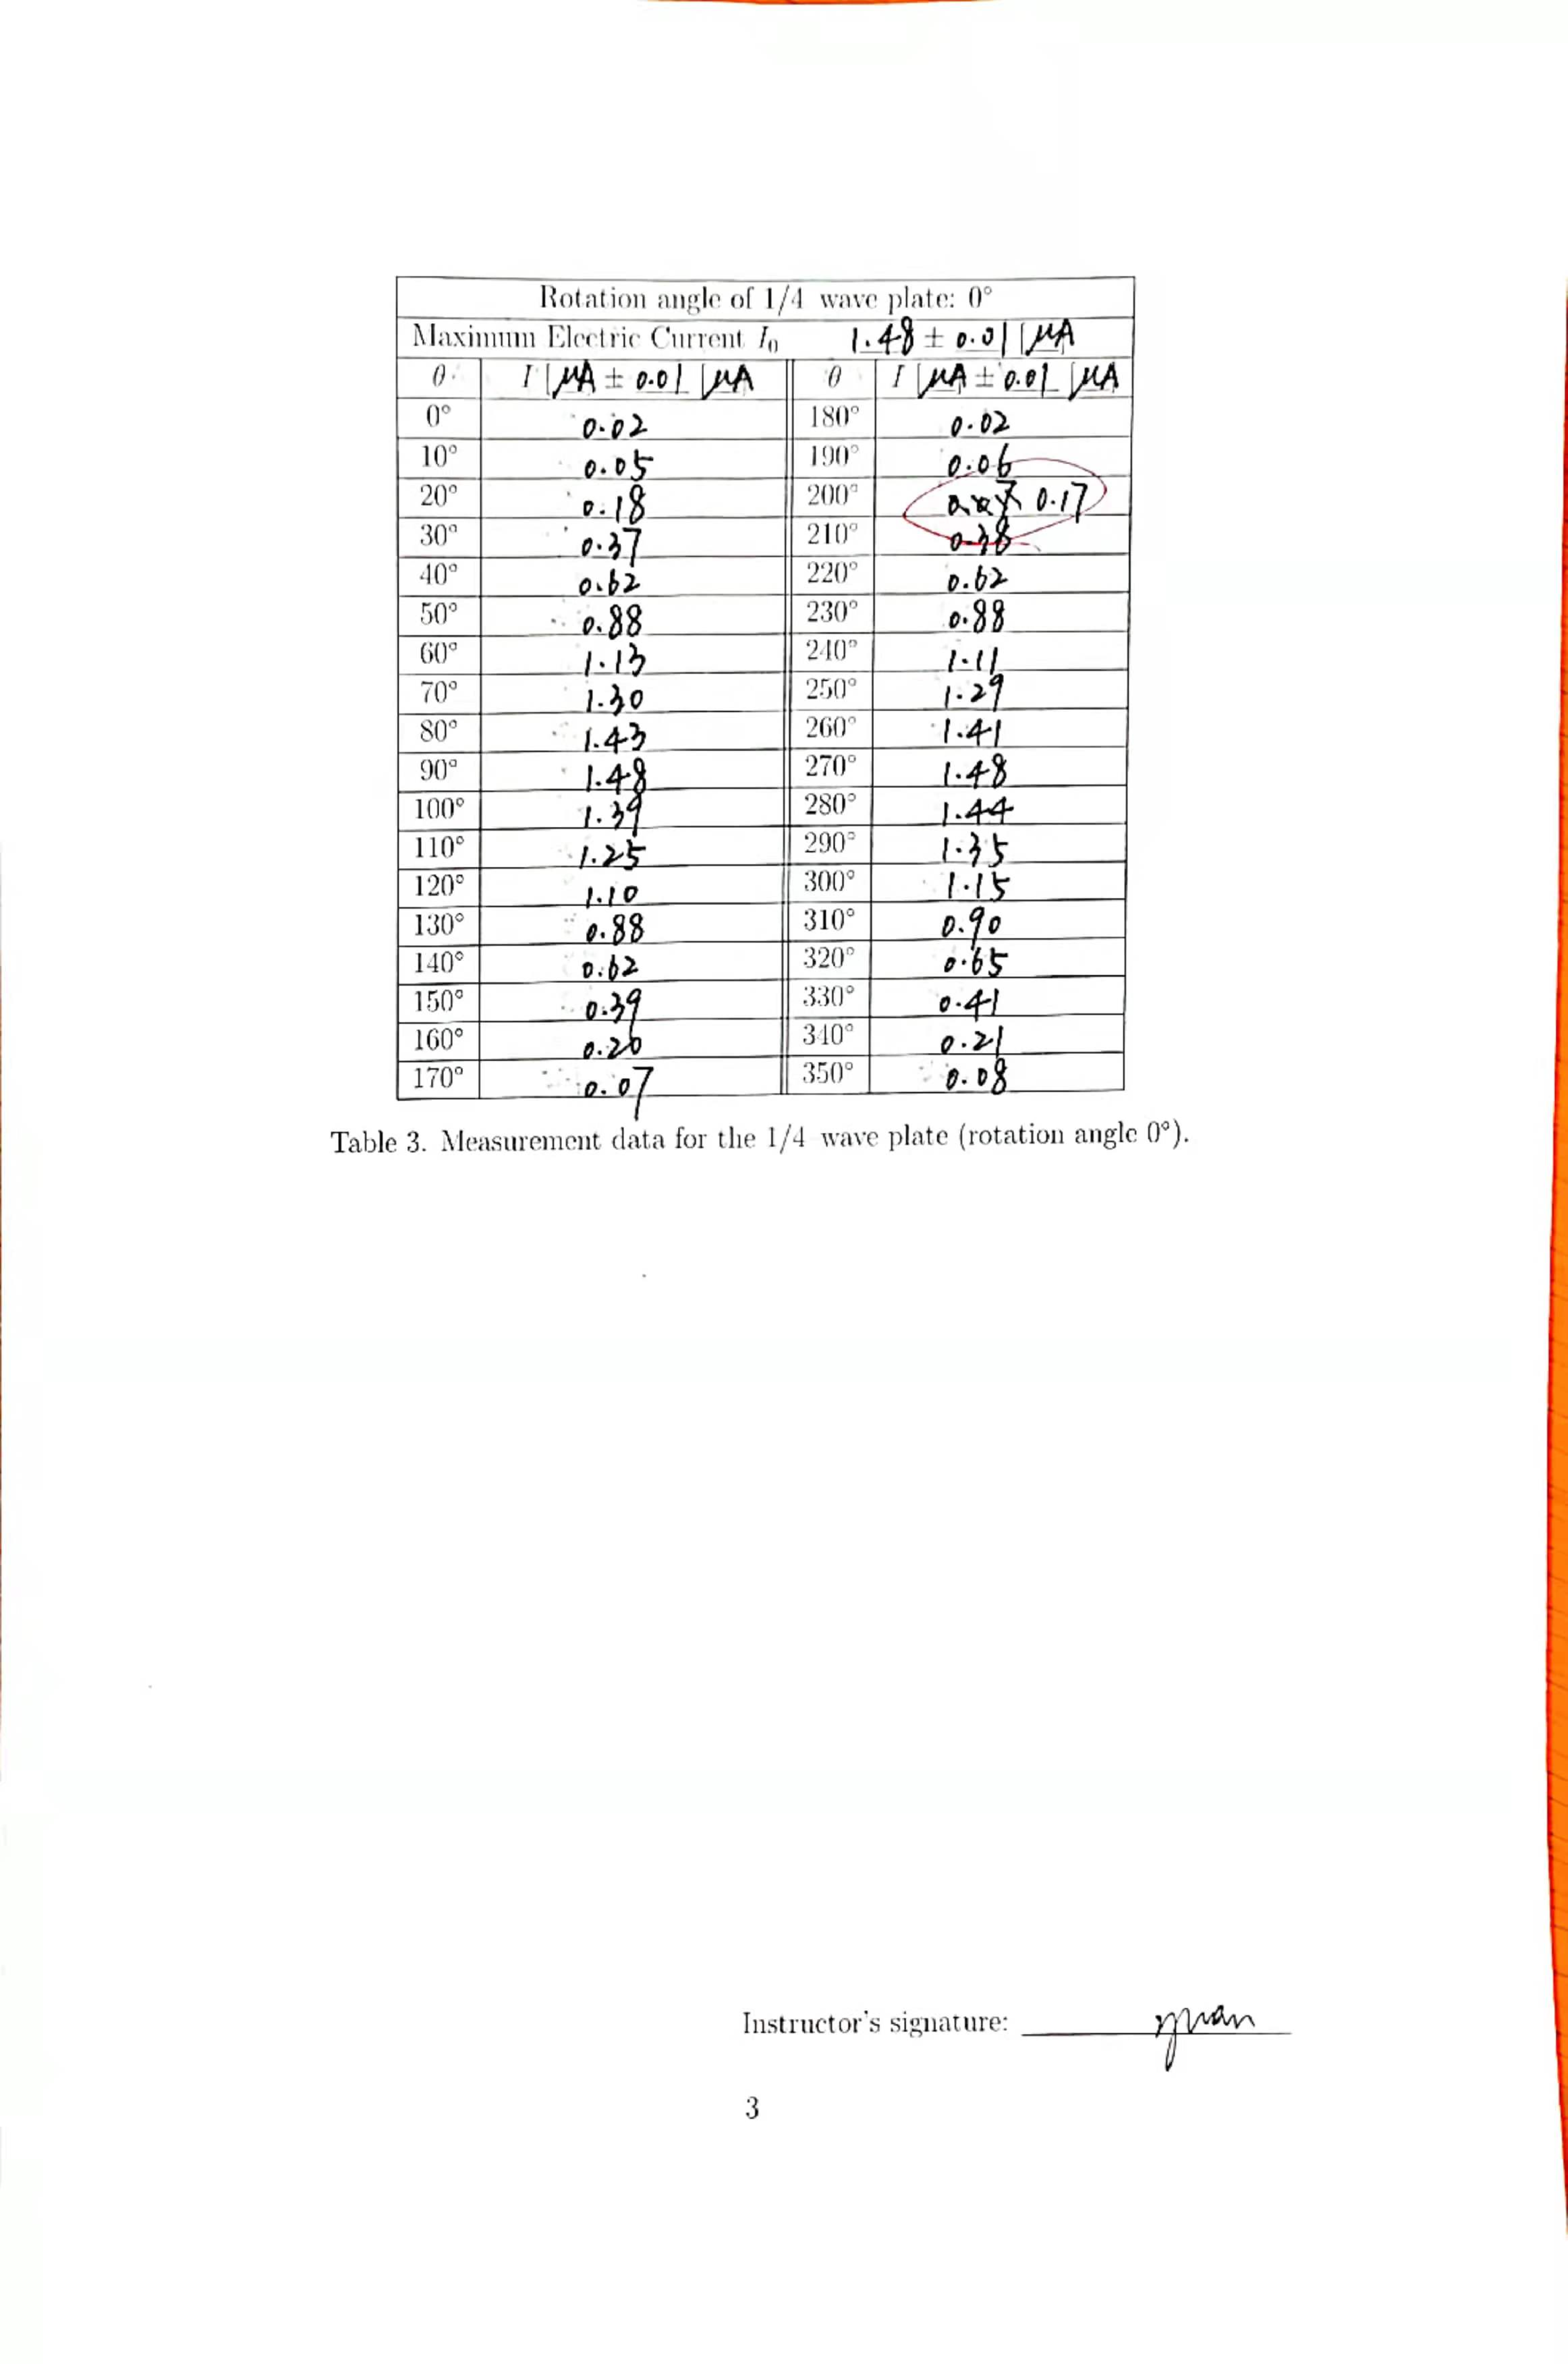
\includepdf{data_sheet3.pdf}
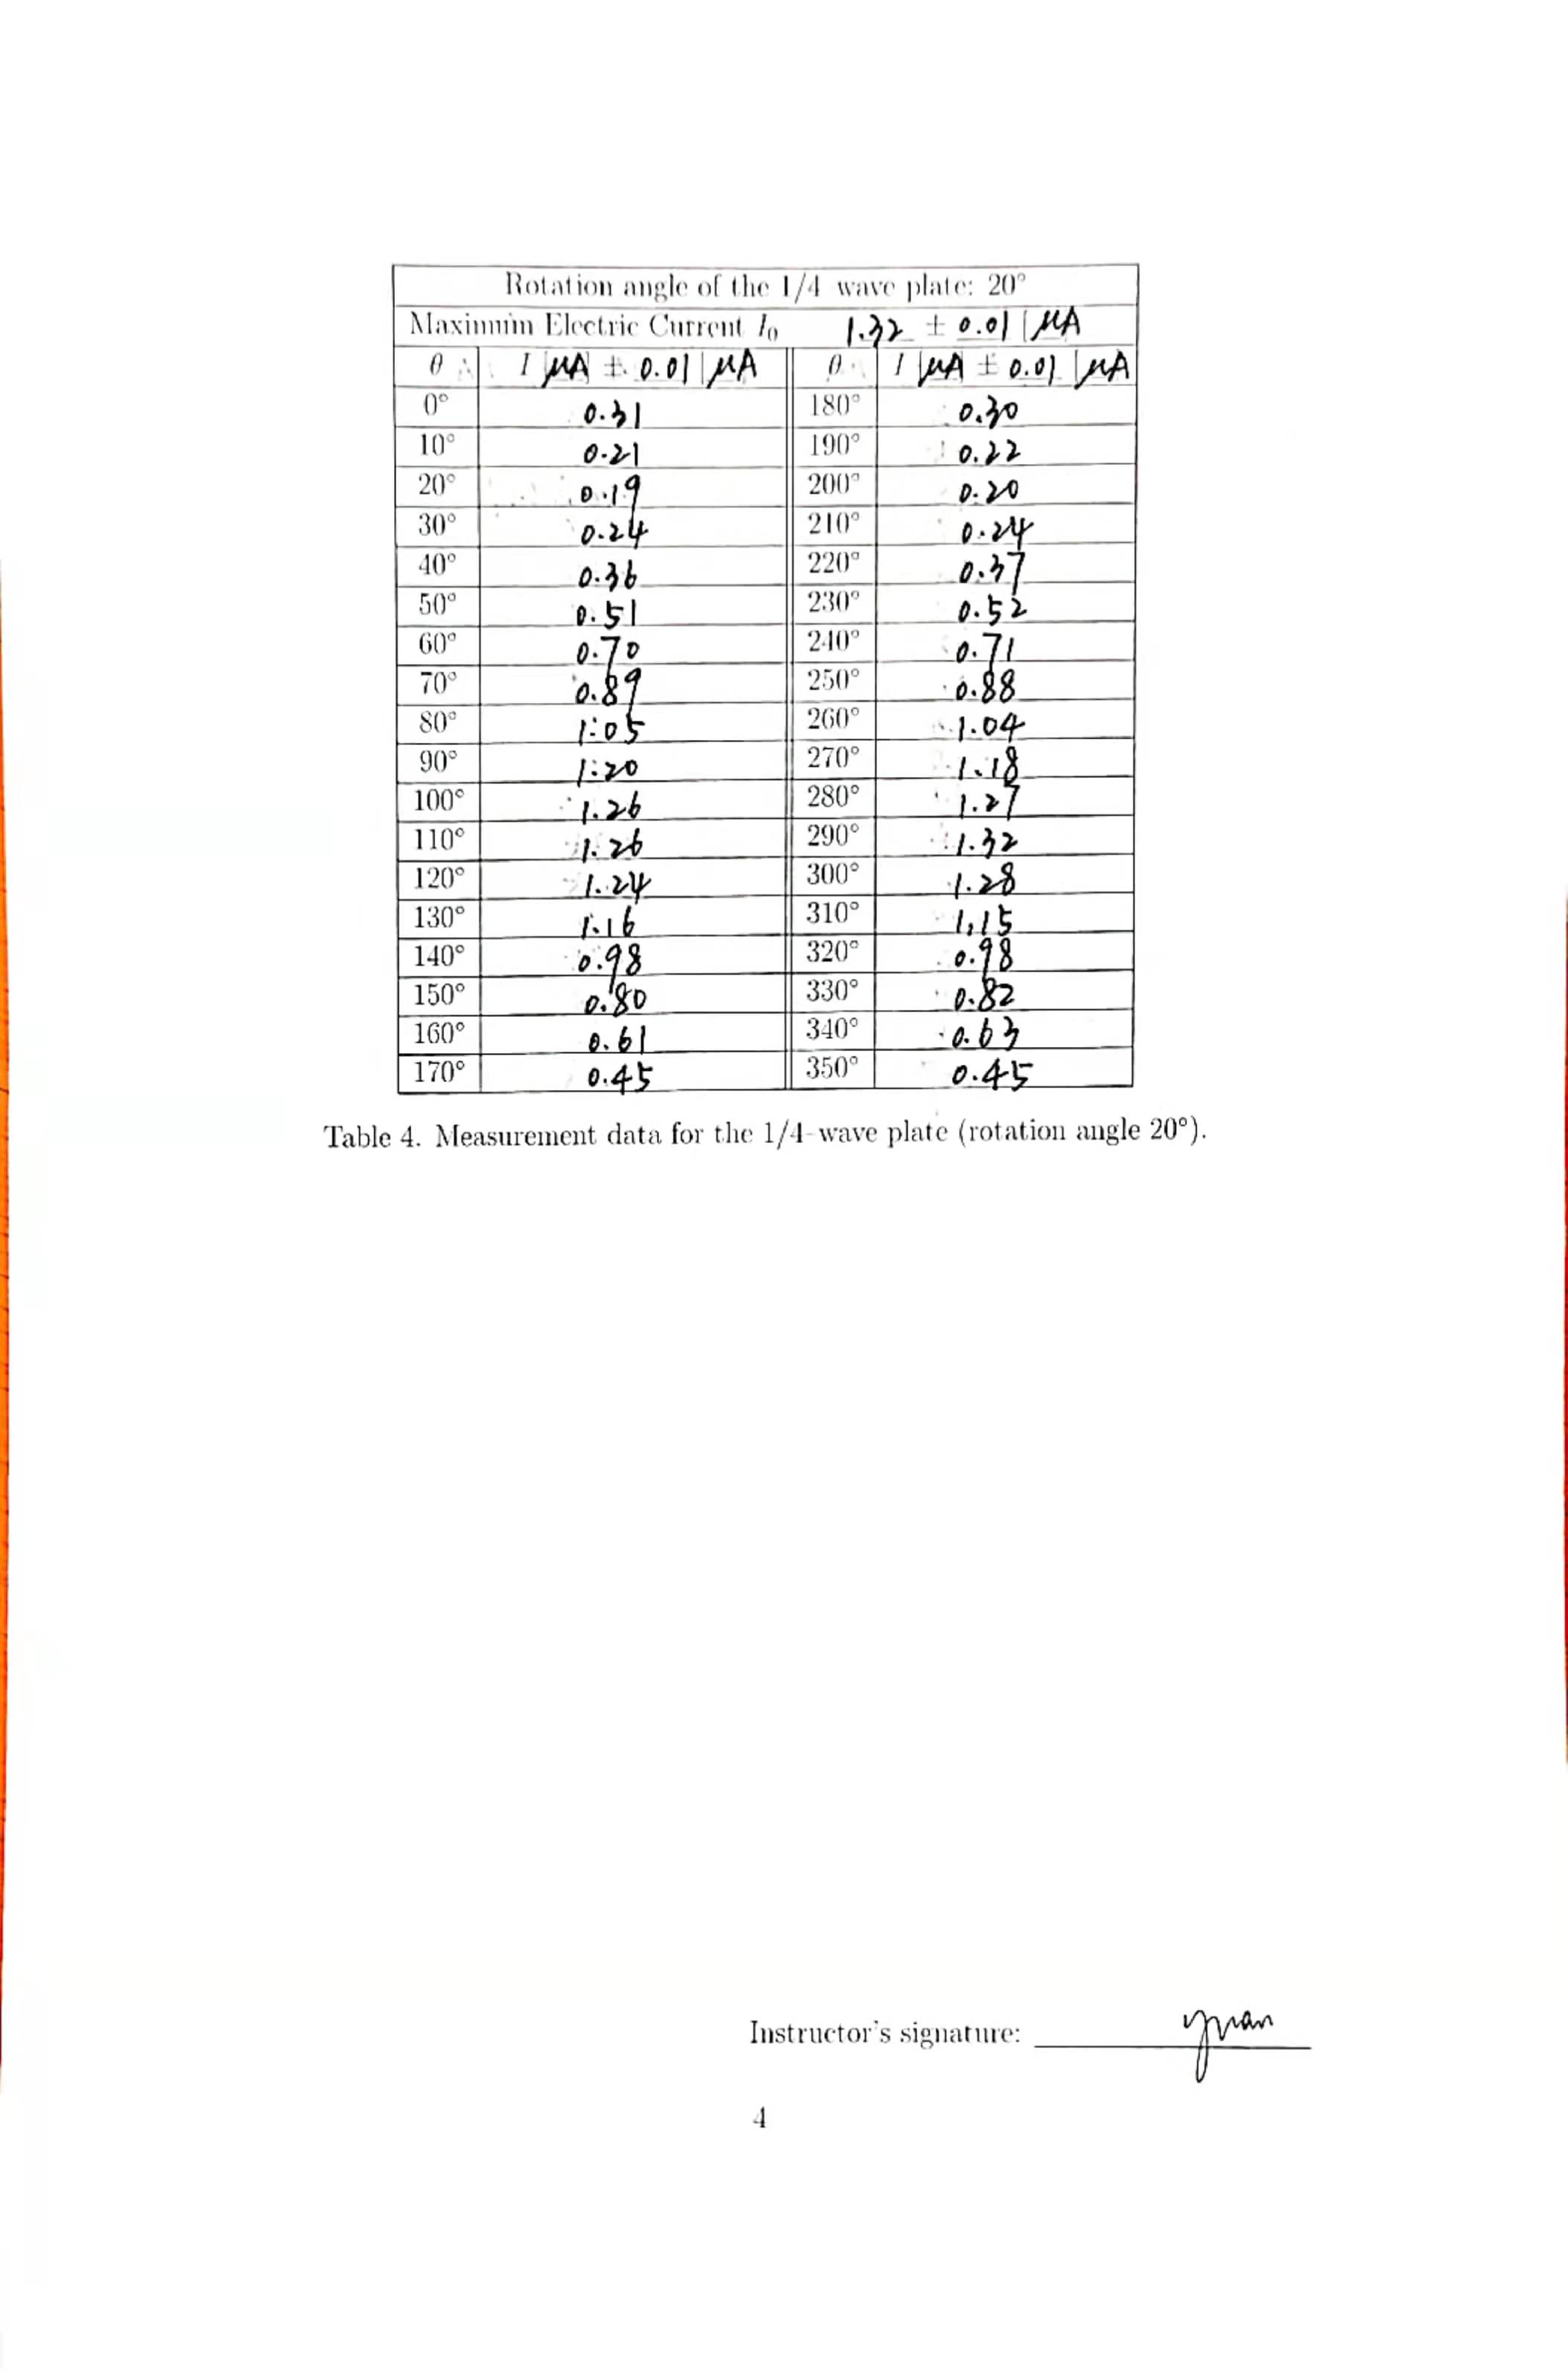
\includepdf{data_sheet4.pdf}
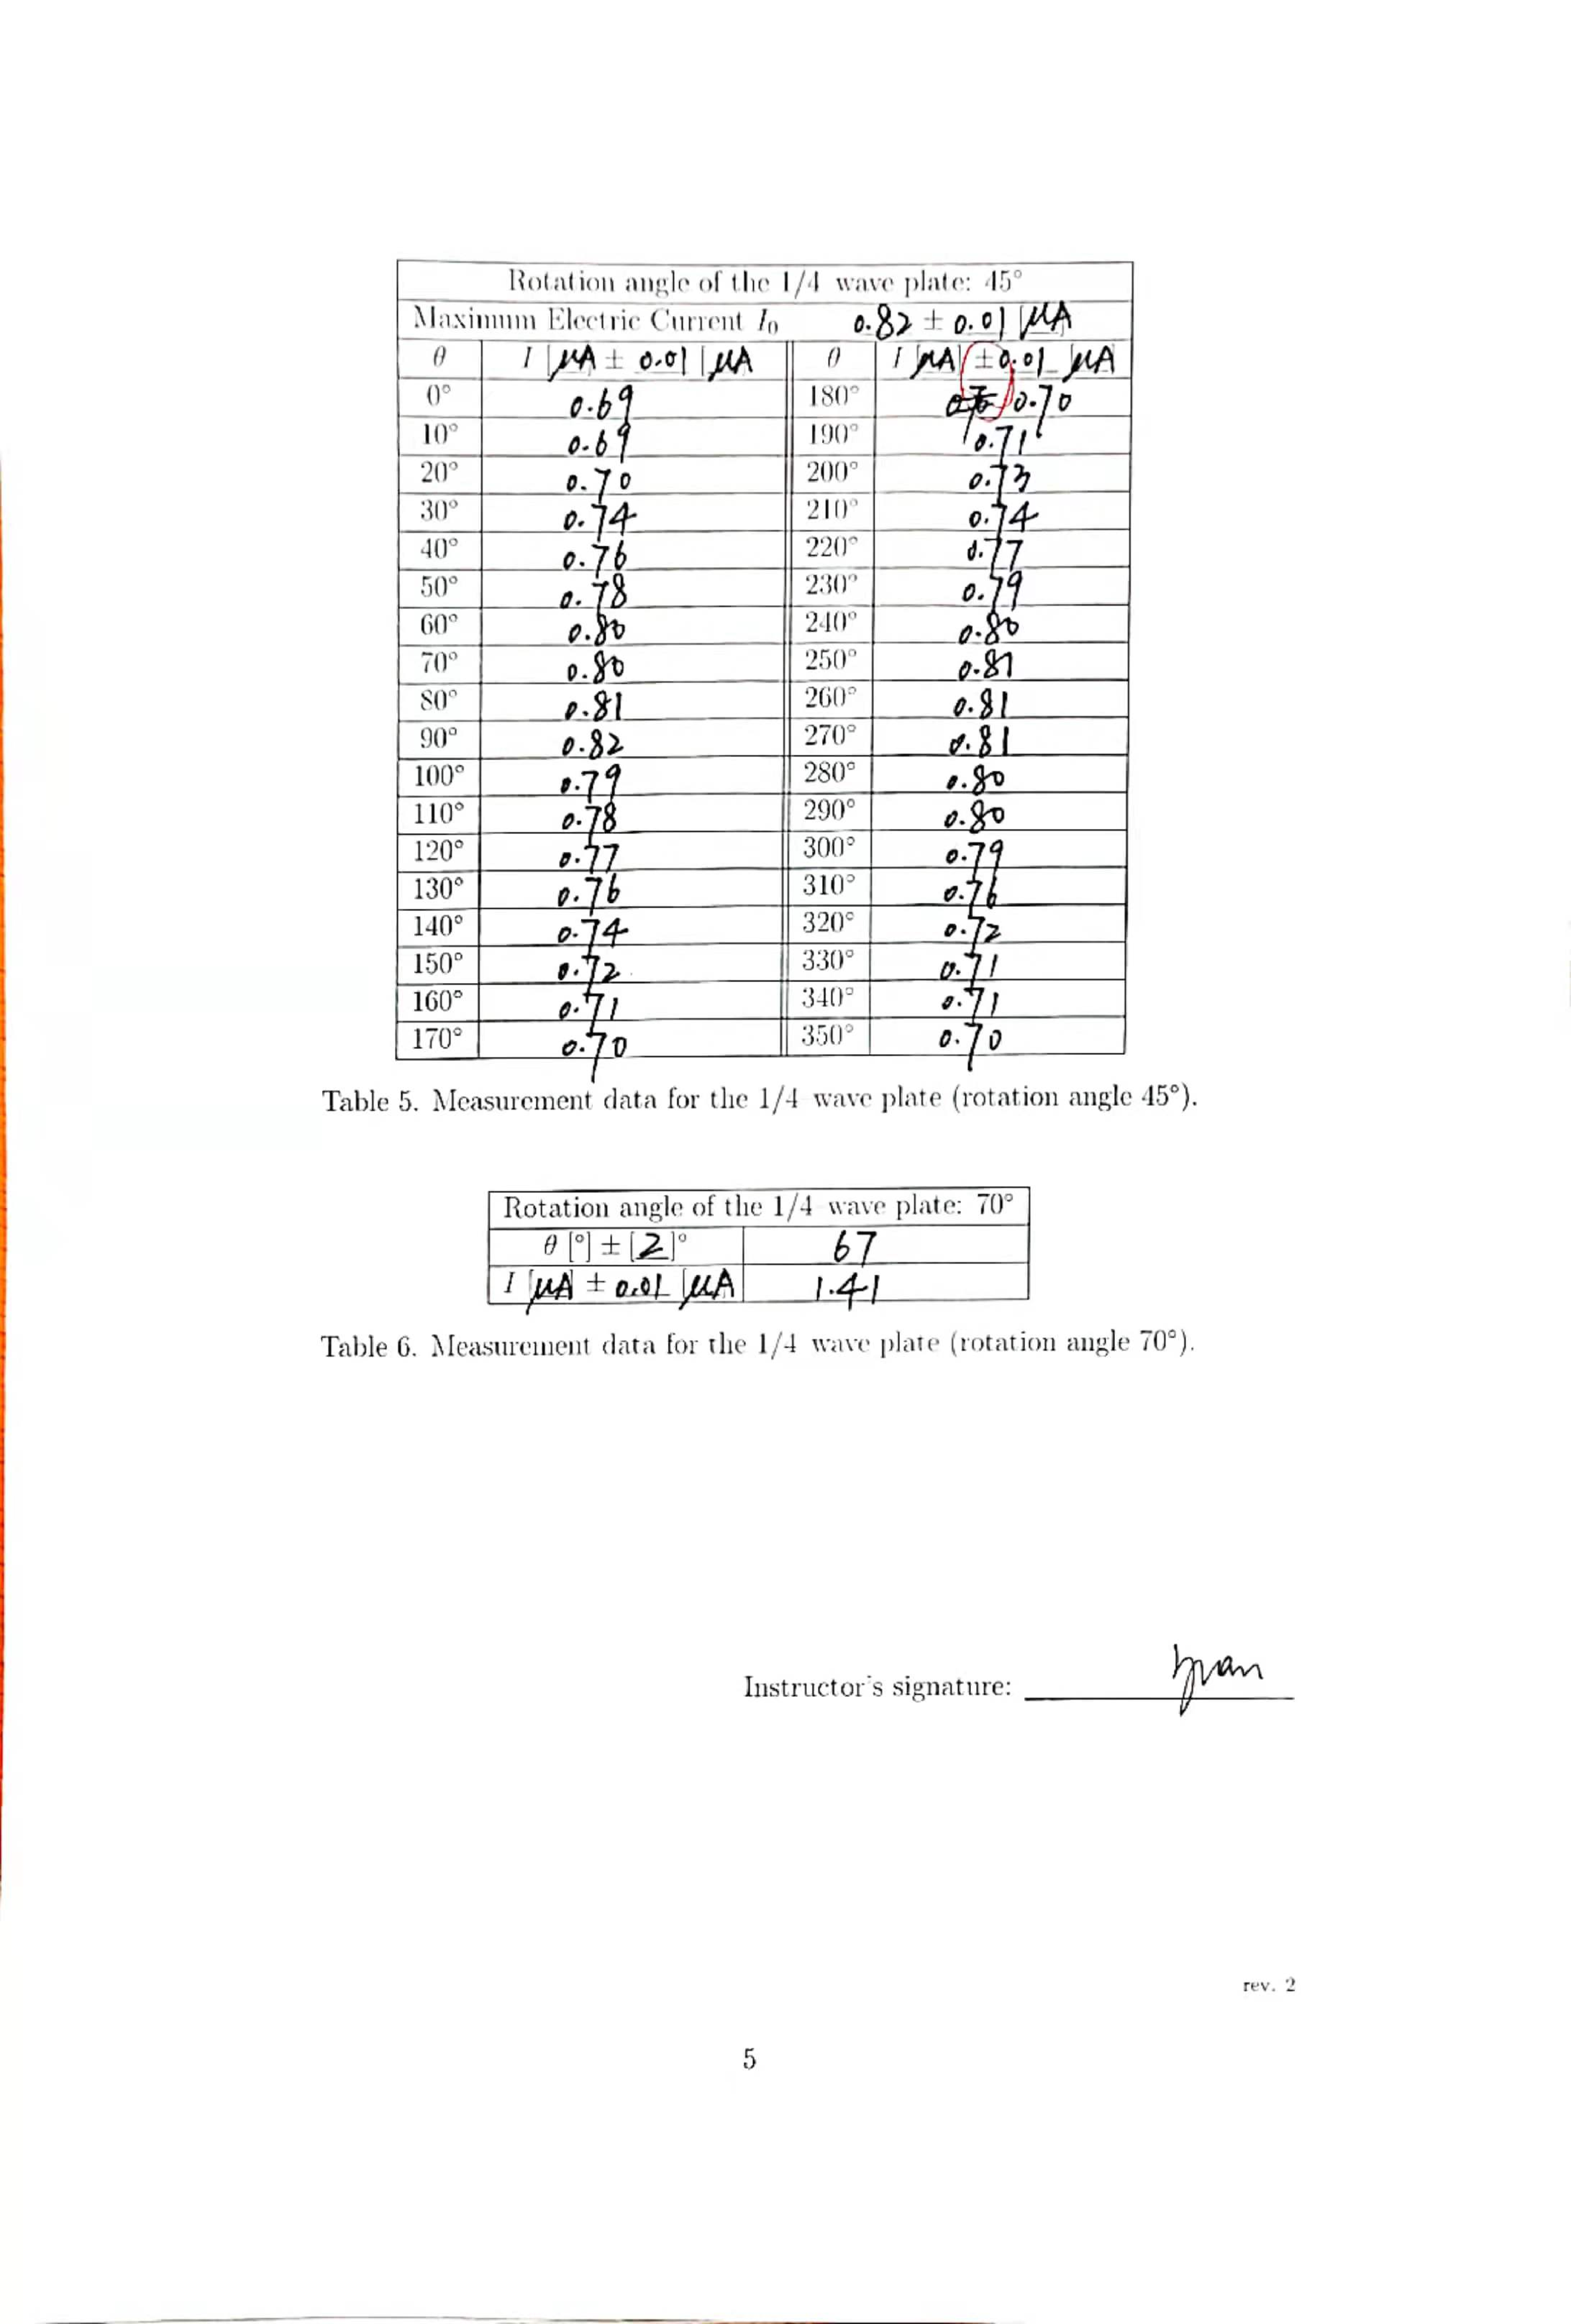
\includepdf{data_sheet5.pdf}

\end{document}
